\documentclass[parskip=full]{scrartcl}
\usepackage[utf8]{inputenc} % use utf8 file encoding for TeX sources
\usepackage[T1]{fontenc}    % avoid garbled Unicode text in pdf
\usepackage[german, english]{babel}  % german hyphenation, quotes, etc
\usepackage{graphicx}       % provides commands for including figures
\usepackage{rotating}
\usepackage{amsmath}
\usepackage{pdfpages}
\graphicspath{ {images/} }
\usepackage{hyperref}       % detailed hyperlink/pdf configuration
\hypersetup{                % ‘texdoc hyperref‘ for options
pdftitle={PSE : LAMeetsML},%
bookmarks=true,%
}
\usepackage{csquotes}       % provides \enquote{} macro for "quotes"
\usepackage[nonumberlist, acronym]{glossaries} % provides glossary commands
\usepackage{enumitem}
\usepackage{lscape}
\usepackage{caption}
%\usepackage{placeins}
\usepackage[section]{placeins}


\makenoidxglossaries
%
%%Glossary
%


\newglossaryentry{ginkgo}
{
	name=ginkgo,
	plural=ginkgo,
	description={The ginkgo libarary is a  c++ libary which among other things enables an user to solve a linear system with a specified \gls{iterative solver} and \gls{preconditioner}. We will be using this libary to solve our systems.}
}
\newglossaryentry{strategy}
{
	name=strategy,
	plural=strategy,
	description={\gls{strategy} is a design pattern of the category behavioral design patterns. It defines a family of iterchangable algorithms. It furthermore enables the selection of an algorithm at runtime, so that the algorithm may vary independently of the clients that use them.}
}
\newglossaryentry{memento}
{
	name=memento,
	plural=memento,
	description={Memento is a design pattern which provides the ability to restore an object to its previous state. In our case the object is the neural network. After a certain amount of training steps we will save the state of the neural network. If the programm crashes at a certain point in time we will be able to reset the state of a neural network to a safed state. That way we will not loose much of our training achievements.}
}

\newglossaryentry{preconditioner}
{
	name=preconditioner,
	plural=preconditioners,
	description={A \gls{preconditioner} is a Transformation of a linear System. With certain \gls{preconditioner}s, certain \gls{iterative solver}s may solve a linear system faster that with no \gls{preconditioner}. The transformation of the \gls{preconditioner} gets applied in each step of the \gls{iterative solver}.}
}
\newglossaryentry{iterative solver}
{
	name=iterative solver,
	plural=iterative solvers,
	description={An \gls{iterative solver} is a method for solving a linear system. An \gls{iterative solver} uses an iterative approach to solve a matrix. An iterative approach is characterized by the idea that the matrix gets solved step by step, where the solution of one step enables the solution of the next step. An \gls{iterative solver} may use a \gls{preconditioner} to improve its results.}
}
\newglossaryentry{tupel}
{
	name=tupel,
	plural=tupel,
	description={A tupel is a structure of data, that holds more than one data, in contrast to other data structures that usually hold only one data.}
}
\newglossaryentry{label}
{
	name=label,
	plural=labels,
	description={A label is a word or a phrase that is used to describe the characteristics or qualities of something}
}
\newglossaryentry{default neural network}
{
	name=default neural network,
	plural=default neural network,
	description={The default neural network is the network we will be using if the user does not specify a different architecture. It will be a Convolutional neural network}
}

\begin{document}

\begin{titlepage}
\centering
{\scshape\LARGE Karlsruher Institut für Technologie\par}
\vspace{1cm}
{\scshape\Large Design Document\par}
\vspace{1.5cm}
{\huge\bfseries Numerical Linear Algebra meets Machine Learning \par}
\vspace {2cm}

{\Large\itshape Fabian Koffer\par}
{\Large\itshape Simon Hanselmann\par}
{\Large\itshape Yannick Funk\par}
{\Large\itshape Dennis Leon Gr\"{o}tzinger\par}
{\Large\itshape Anna Katharina Ricker\par}

\vfill
Supervisors\par
Hartwig Anzt
Makus G\"{o}tz

\vfill
{\large\today\par}
\end{titlepage}

\tableofcontents
\newpage

\section{Overview}

%include big class diagramm

\section{Module Interaction}

\subsection{Class Descriptions}

\subsubsection{Class CommandLineInterface}
The class CommandLineInterface represents the concrete command line interface. 
Therefore it only consists of two methods. 
The first one is read\char`_input that receives a message that will be displayed and reads the next user input. 
The other method is create\char`_output. 
This method prints a string to the CLI.

\subsubsection{Class Controller} 
The controller is the main entry point for the program execution. 
It creates the view, receives the user input, calls the parser to create a command from the input and starts the module the user wants.

\subsubsection{Class CommandParser}
The CommandParser is a static class that gets the input which the user entered and parses it to a concrete command-object.

\subsubsection{Class Command}
The Command class holds all the information entered by the user that is needed to execute a module.
There is one command subclass for each module and the command class also validates that all parameters are available to run the module.
The command also has a execute method which runs the specific module with all the arguments it needs.


\subsection{Activity Diagrams}

\subsubsection{User Input Activity Diagram}

This activity diagram shows the main workflow of the whole program.
The program first waits for user input.
After the user enters his input into the command line interface, the CommandParser parses this input to a command.
If the command equals quit, the program will exit.
If not the command will be validated to contain enough information to start the desired module.
If it is not valid, an error message will be printed and the user can enter a new input.
If the command is valid, the module will be started.
Therefore the module computes his specific task in iterations.
After each iteration it prints the current progress to the user.
This two activities repeat until all tasks are done.
When the module is finished, the program prints a complete message and starts waiting for new user input.

\newpage

\begin{figure}[h]
\begin{center}
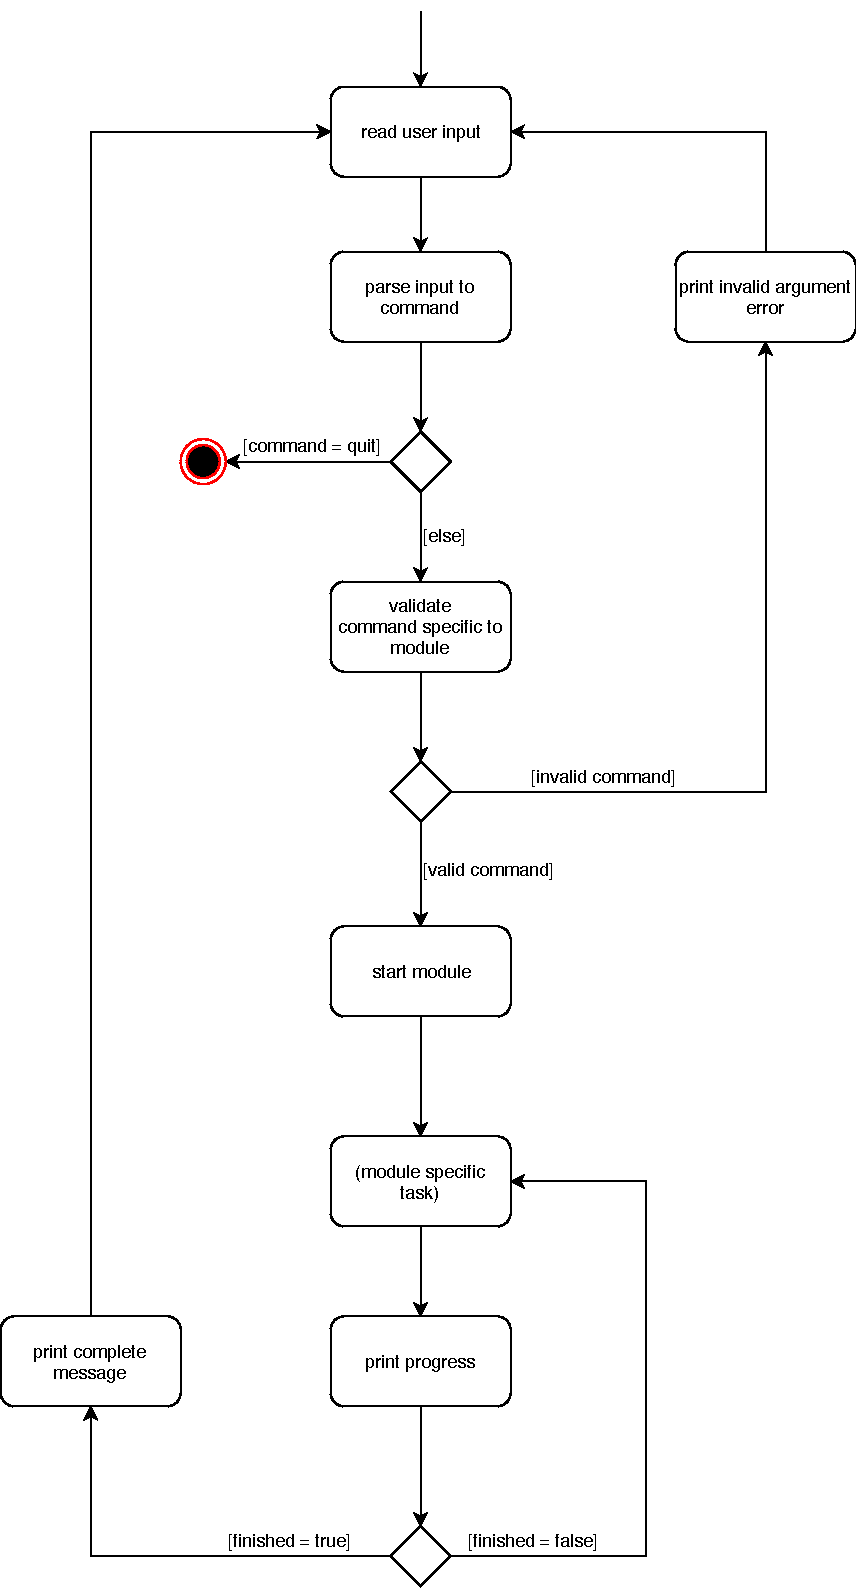
\includepdf[width=\textwidth, height= \textheight, keepaspectratio]{ActivityDiagrams/PDF/user_input_activity_diagram}
\label{User Input Activity Diagram}
\end{center}
\end{figure}
\newpage

\subsection{Class Diagrams}

\subsubsection{Command Parsing}

This class diagrams shows all classes that are used by the CommandParser.
The CommandParser has one method that receives an input string and returns a command.
This method uses the first word of the input string to determine which module is supposed to be started.
Based on this he creates an instance of this subclass of the command.
The remaining string will be parsed to a dictionary with keys and values. 
This dictionary is passed to the constructor of the command object.
In the constructor of the command, the command also calls the validate() method.
This method checks if all arguments that are necessary for the specific module start are provided.
After that is finished the command can be returned by the CommandParser.
The execute method of the command can be then used to start the modules computation.

\newpage

\begin{figure}[h]
\begin{center}
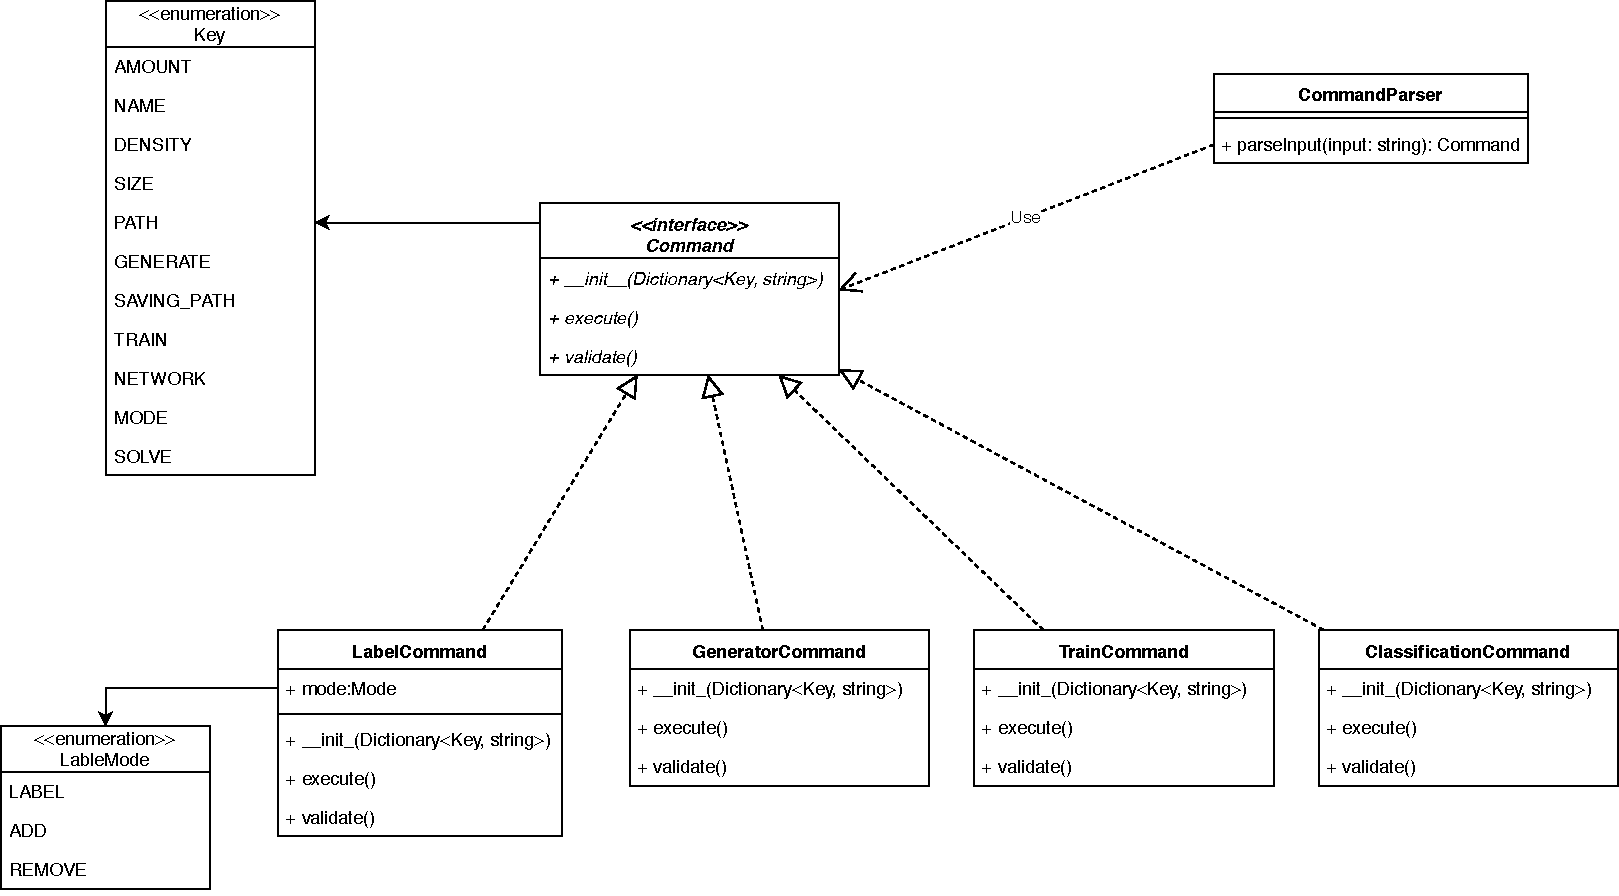
\includepdf[width=\textwidth, height= \textheight, keepaspectratio]{ClassDiagrams/PDF/CommandParsing}
\label{Command Parsing}
\end{center}
\end{figure}
\newpage

\subsection{Component Diagram}

\subsubsection{Model View Controller Component Diagram}

This component diagram shows the main interaction between the modules.
For our main structure we use the model view controller
Each class belongs to one of the three parts: view, controller or model.
In the view there is the CommandLineInterface, which as the name suggests represents the command line.
It receives strings, that it will display and makes the user input available for other classes.
The other class in the view is the CLIOutputService.
This class works as the observer for the model and receives the strings the model wants to output.
It then provides strings that can be displayed by the command line interface.

The next big part is the controller.
This parts main component is the class that is also called controller.
This class gets a string by the CommandLineInterface.
This string it then passed to the CommandParser.
This class creates the right command and passes the arguments to this command.
The command stores this arguments and makes them available for the modules.

The model consists of the four static modules that make the computations.
This modules get the arguments that are provided by the command.
The modules can also provide strings that can be displayed in the view.

\newpage
\begin{figure}[h]
\begin{center}
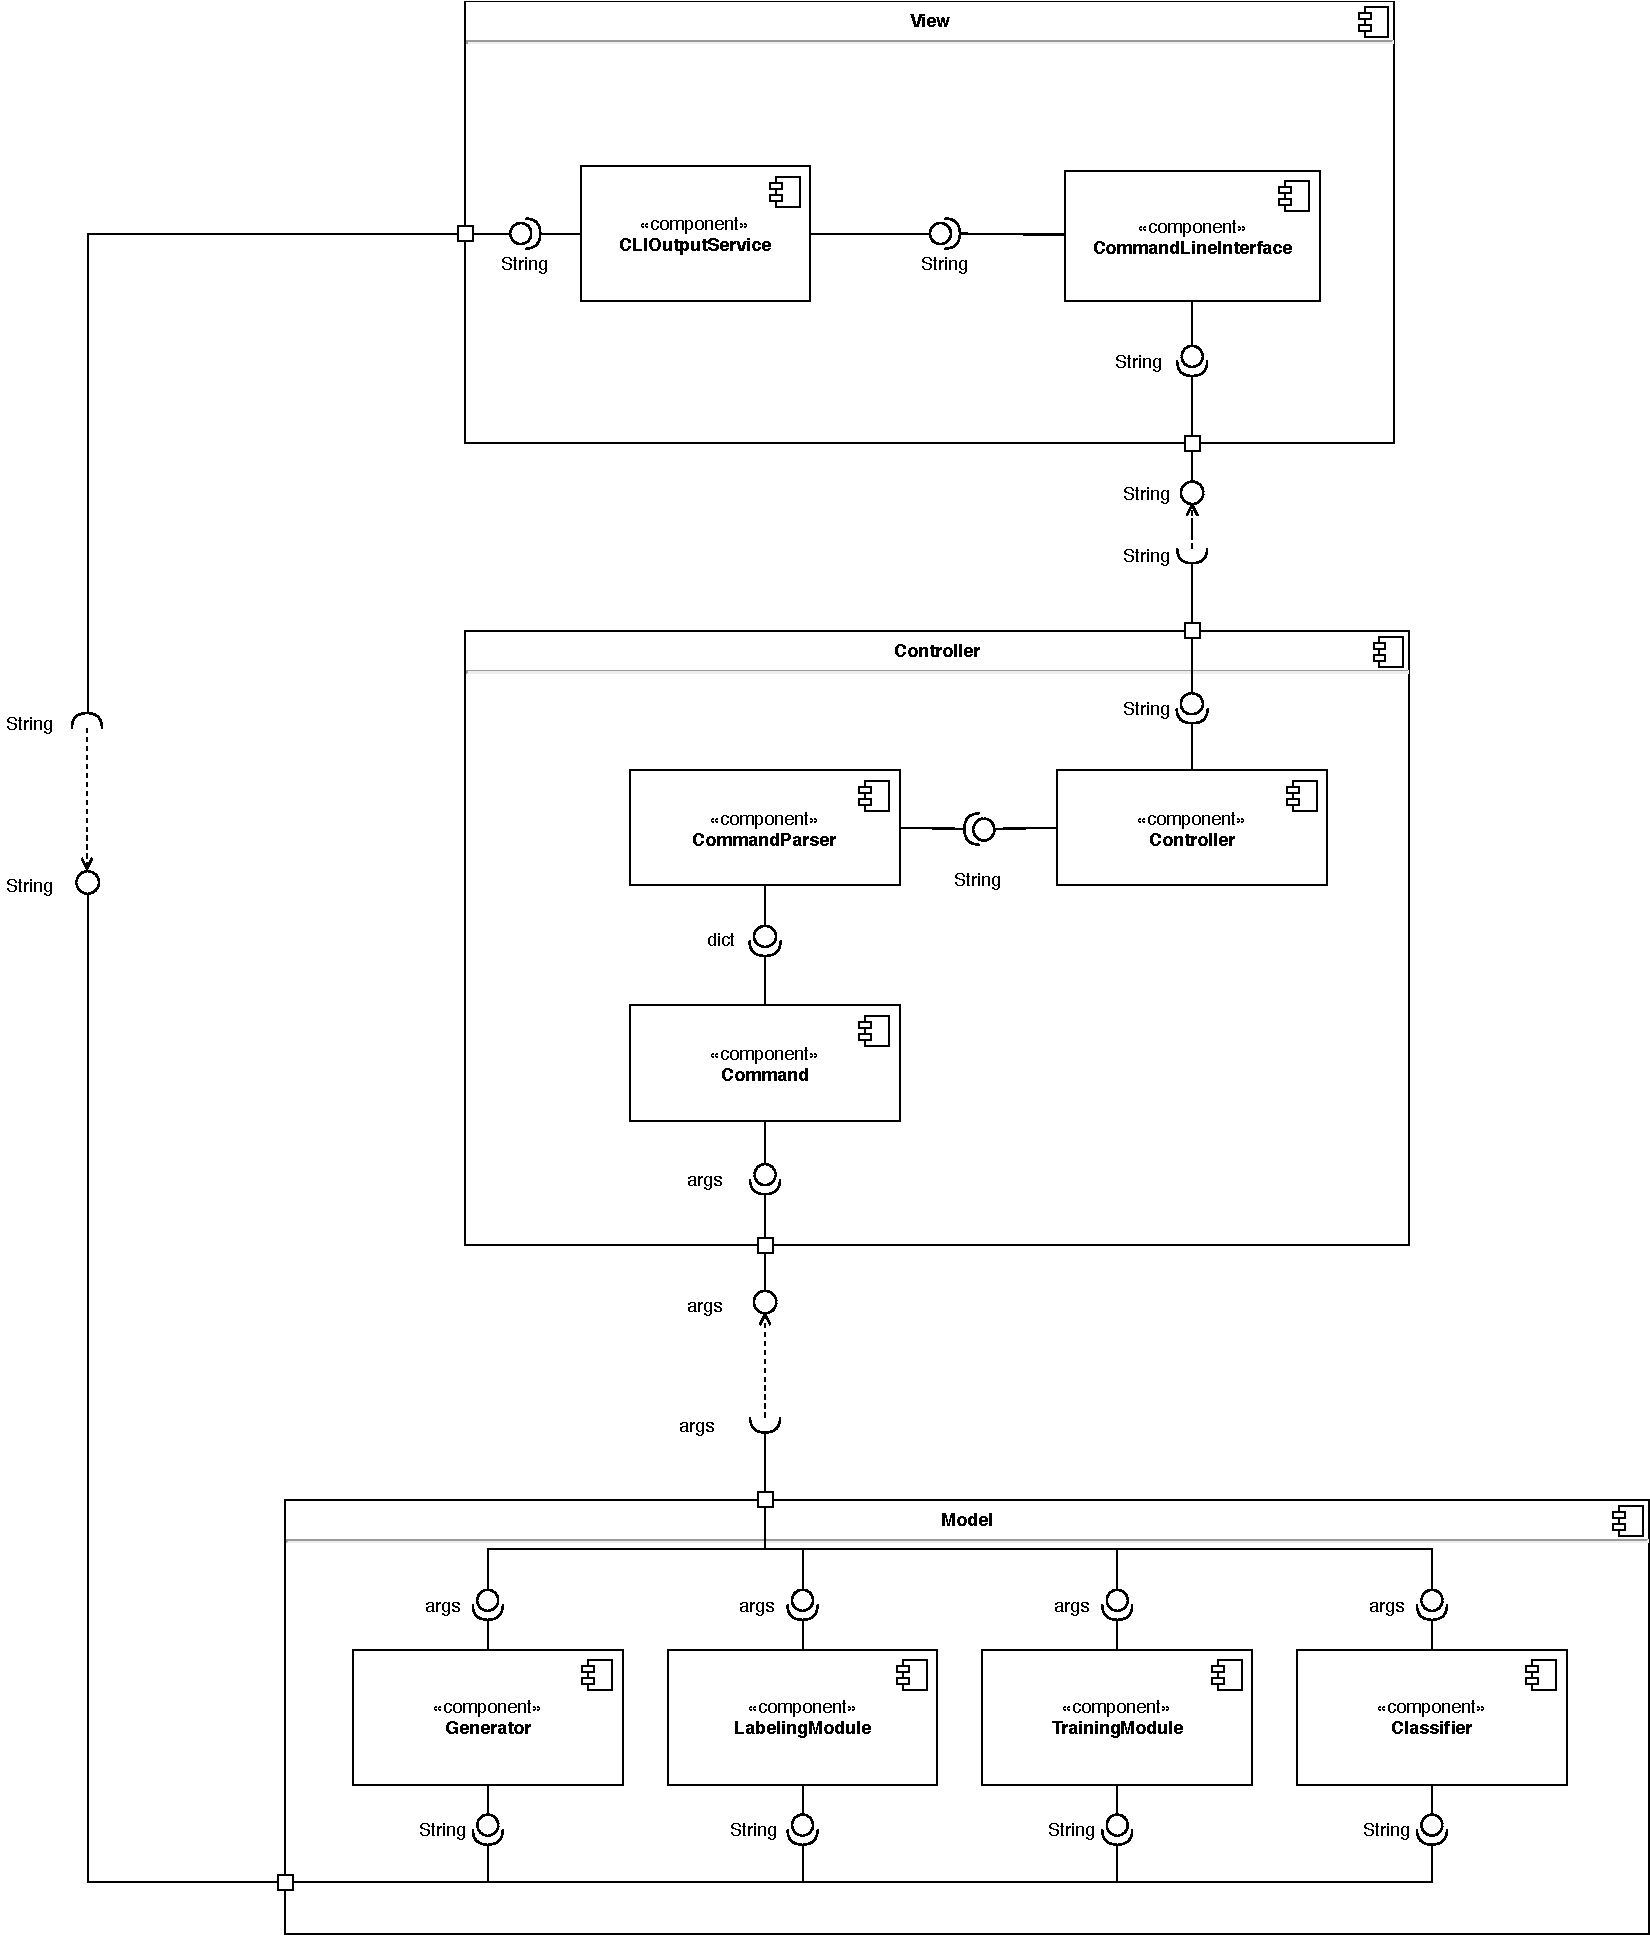
\includepdf[width=\textwidth, height= \textheight, keepaspectratio]{ComponentDiagrams/PDF/interaction_overview}
\label{Model View Controller Component Diagram}
\end{center}
\end{figure}
\newpage


\subsection{Sequence Diagrams}

\subsubsection{Controller Sequence Diagram}

This class diagram shows what happens when the controller is being created.
First it will create the CommandLineInterface class.
After finishing that, it asks the command line interface for user input.
This user input is then passed to the CommandParser that creates a dict out of this string and creates the right instance of a Command.
When creating a command, it also calls the validate method that checks if all arguments that are needed by the module for running its computation are provided.
If thats the case, the controller creates a CLIOutputService and attaches the CommandLineInterface to it.
This CLIOutputService is then registered to the module so this can create output to the command line interface.
After all this setup steps, the module is ready to be executed.
Therefore the controller calls the execute method on the command, which then calls the start method of the module with the arguments it needs.
The module then starts its computations and eventually calls the CLIOutputService to create some user output.
The module calls print\char`_line with the string it wants to output.
The CLIOutputService creates the string that can be displayed and this is passed to the CommandLineInterface that is attached to CLIOutputService.
After all computations are done, the module returns his call.
Now the user can enter a new input until he enters quit.

\newpage
\begin{figure}[h]
\begin{center}
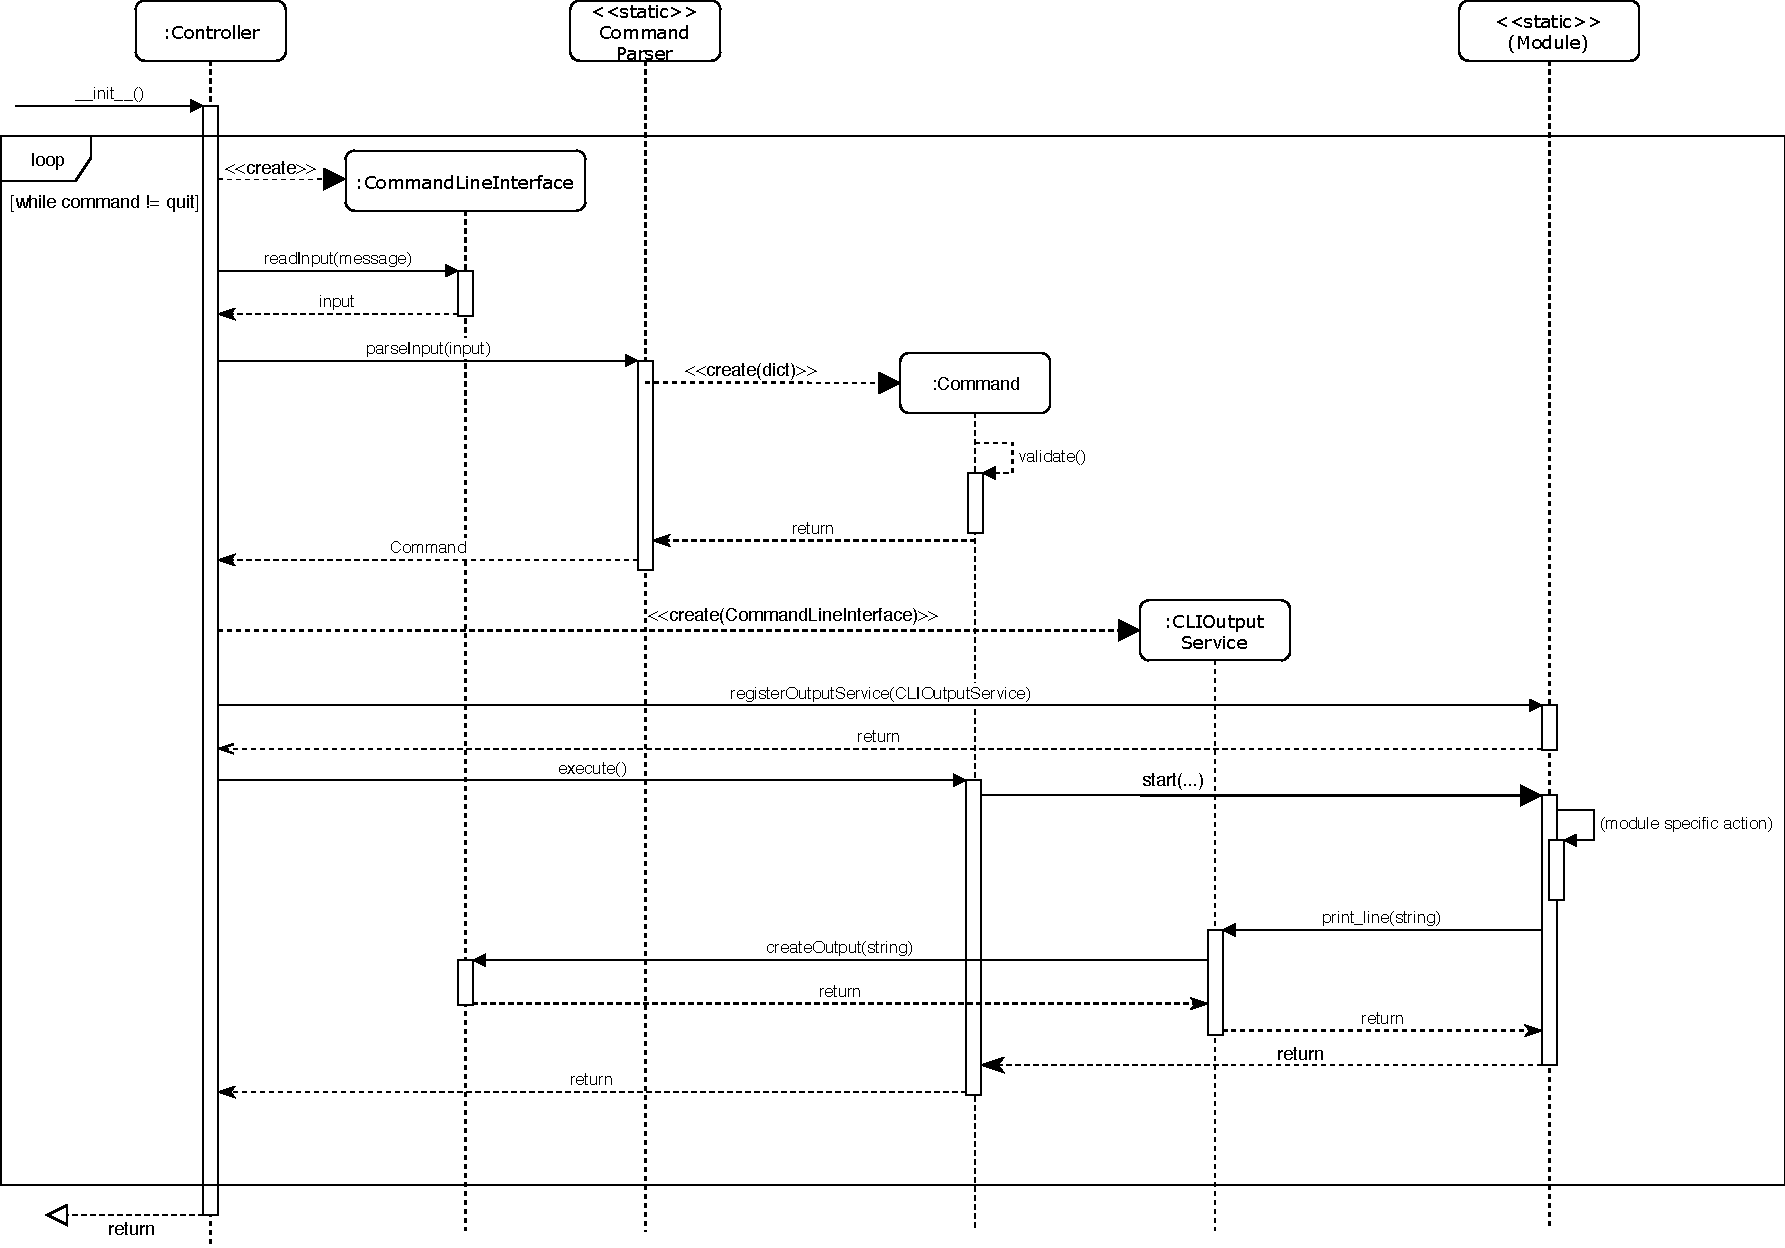
\includepdf[width=\textwidth, height= \textheight, keepaspectratio]{SequenceDiagram/PDF/controller_sequence_diagram}
\label{Controller Sequence Diagram}
\end{center}
\end{figure}
\newpage

\section{Display Output}

\subsection{Class Descriptions}

\subsubsection{Interface OutputService}
The OutputService interfaces can be implemented and passed to a module to receive the output of the modules. 
Therefore it has methods that represent different ways output can be displayed. 

 \subsubsection{Interface Subscriber}
The Subscriber interface only provides the method update() which will be triggered by an Observable upon receiving new values.

\subsubsection{Class Observable} 
The Observable class can be used to notify subscribers when new values are provided.
Subscribers can subscribe themselves to an Observer to get notifications about new data.
The next() method calls update() on each subscriber.

\subsection{Class CLIOutputService}
This class implements the OutputService and the Subscriber interface. 
On creation it gets a reference of the CommandLineInterface to which it will pass the lines the modules wants to output.
It also implements the Subscriber interface to subscribe itself to an observable.
This can be used to display lines that are overwritten with new values like an progress bar or a counter.

\subsection{Class Diagrams}

\subsubsection{Command Parsing}

This class diagrams shows all classes that are used by the CommandParser.
The CommandParser has one method that receives an input string and returns a command.
This method uses the first word of the input string to determine which module is supposed to be started.
Based on this he creates an instance of this subclass of the command.
The remaining string will be parsed to a dictionary with keys and values.
This dictionary is passed to the constructor of the command object.
In the constructor of the command, the command also calls the validate() method.
This method checks if all arguments that are necessary for the specific module start are provided.
After that is finished the command can be returned by the CommandParser.
The execute method of the command can be then used to start the modules computation.

\newpage
\begin{figure}[h]
\begin{center}
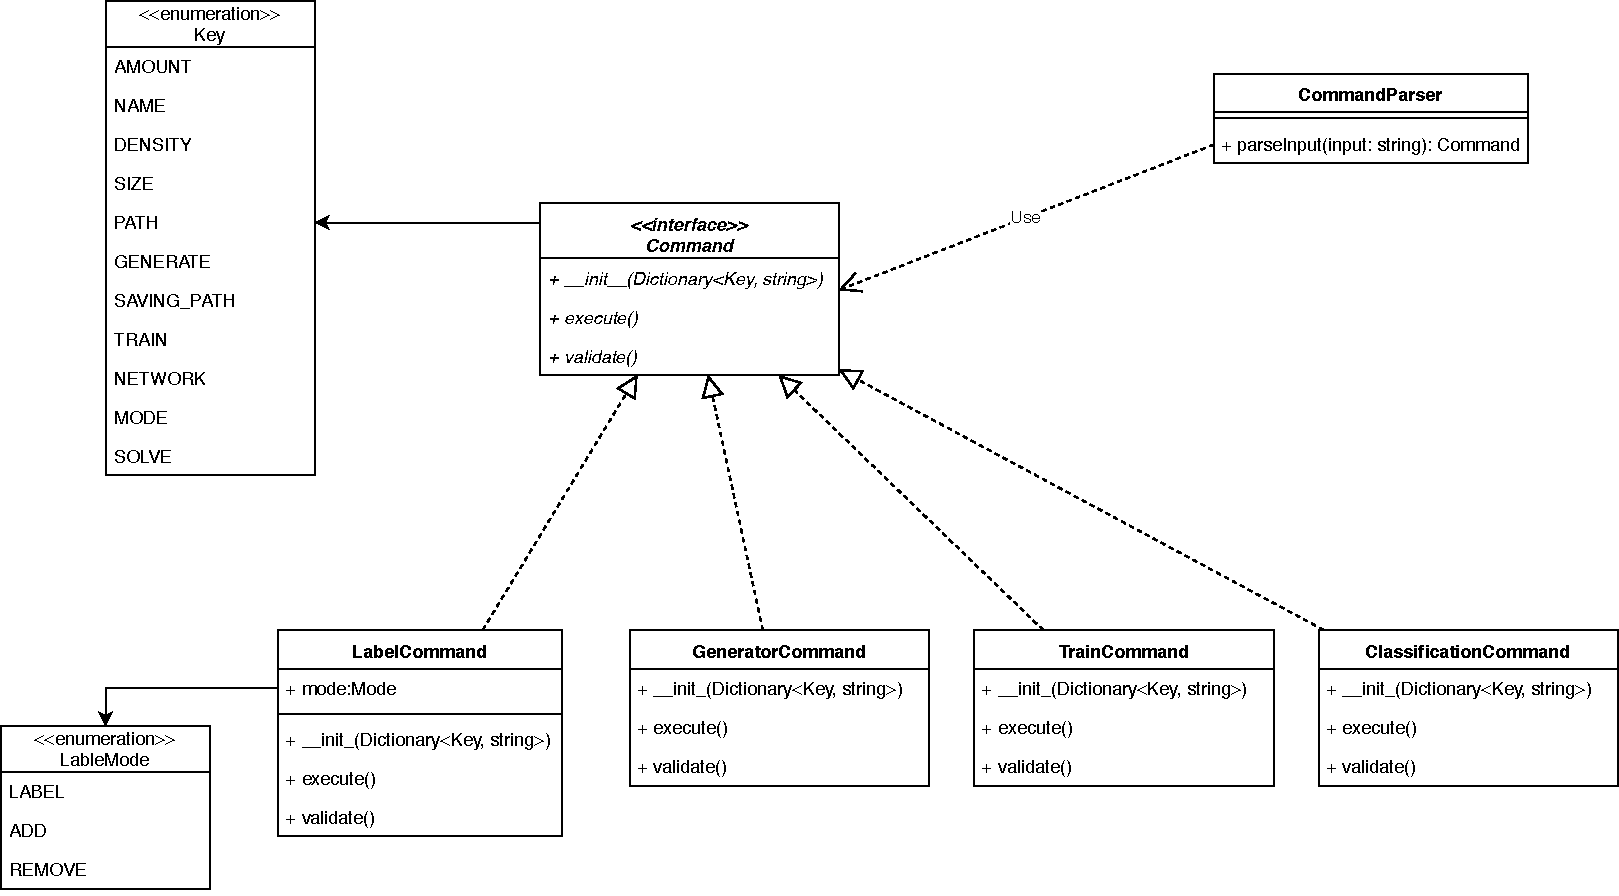
\includepdf[width=\textwidth, height= \textheight, keepaspectratio]{ClassDiagrams/PDF/CommandParsing}
\label{Command Parsing}
\end{center}
\end{figure}
\newpage

\subsection{Sequence Diagrams}

\subsubsection{Print Overriding String}

Sometimes the user wants to print a progress like a download status that is updated by time.
But there should not be a new line for each percentage the download gets further.
Instead the old string should be overwritten by time and and the module should only have to pass the new status.
Therefore there is the method print\char`_overriding in the CLIOutputService that wants an string and an observable object.
That is why the module first creates the observable object.
This object is then being passed to the print\char`_overriding method together with a string that will stay the same for this process.
Because the CLIOUtputService implements the Subscriber interface, it can subscribe itself to the observable.
Now that the CLIOutputService is subscribed to the Observable, it will be notified when the Observable gets new data.
When the module starts it computations, it can call next with the new data with which it wants to override the old one in the view.
In the next call of the observable, all subscribers will be notified with the new value.
The string with the new value can now be printed to the command line interfaces

\newpage
\begin{figure}[h]
\begin{center}
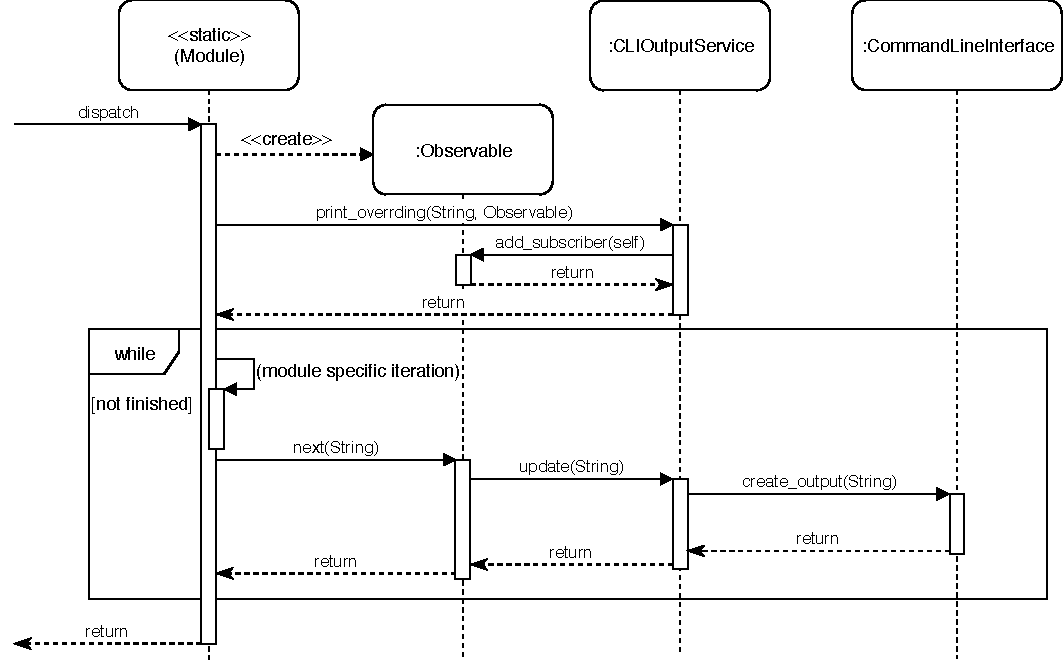
\includepdf[width=\textwidth, height= \textheight, keepaspectratio]{SequenceDiagram/PDF/print_progress_sequence_diagram}
\label{Print Overriding String}
\end{center}
\end{figure}
\newpage

\section{Exception Handling}

\subsection{Class Diagrams}

\subsubsection{Exception Classes}

Each exception extends Python's Exception class.
There are four kinds of exceptions that may be thrown by one of our classes.\newline\newline
The IllegalArgumentException will be thrown if the arguments the user has entered are not valid.\newline\newline
The InvalidConfigException will be thrown if the user edited the configuration file with invalid arguments or syntax.\newline\newline
The IOException will be thrown if errors occur while reading from or writing data to the hard drive.\newline\newline
The InvalidOSException will be thrown if some part of our program is trying to access functionality that is not supported on the current operating system.

\newpage
\begin{figure}[h]
\begin{center}

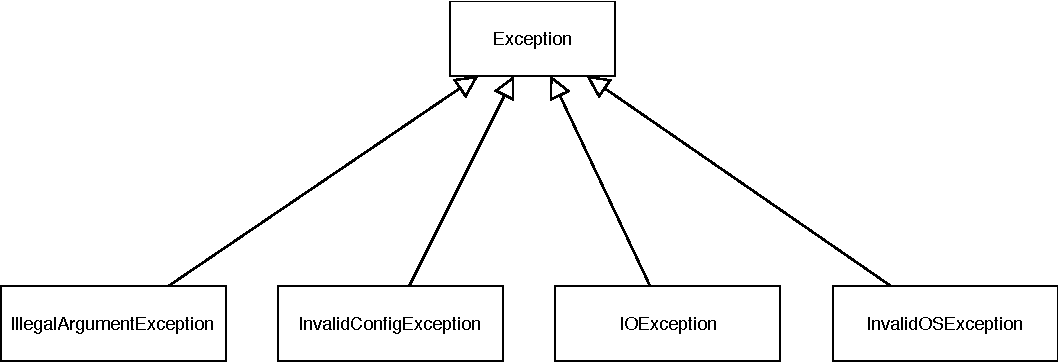
\includepdf[width=\textwidth, height= \textheight, keepaspectratio]{ClassDiagrams/PDF/exception_cases_class_diagram}
\label{Exception Classes}
\end{center}
\end{figure}
\newpage

\section{Collector}
\begin{figure}[h]
\begin{center}
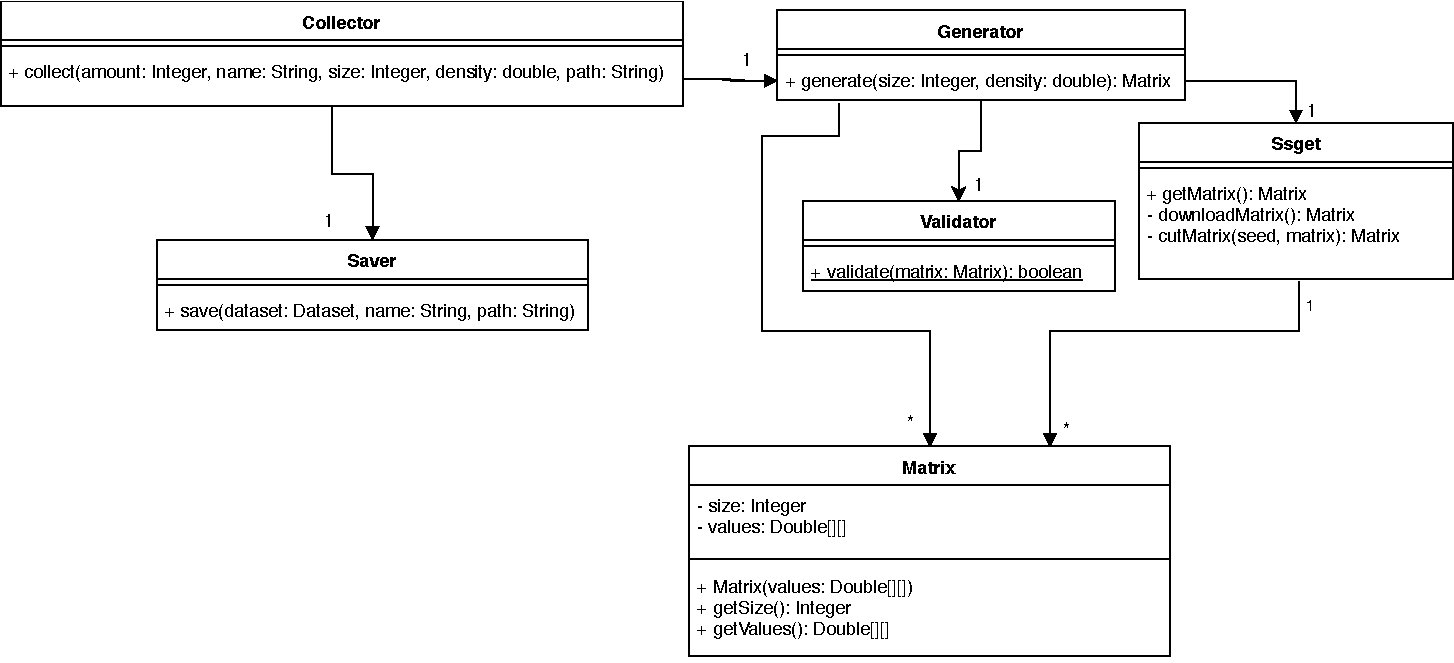
\includegraphics[width=\textwidth, height= \textheight, keepaspectratio]{ClassDiagrams/PDF/Collector_classdiagram.pdf}
%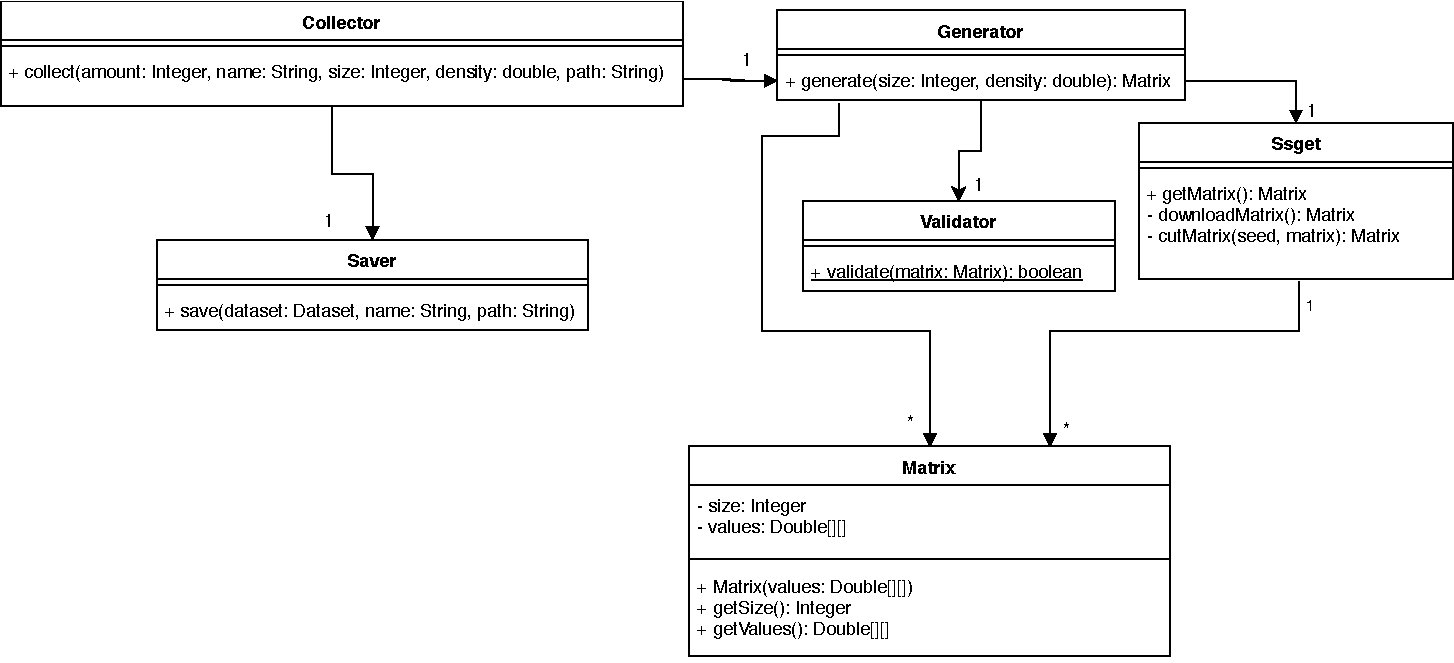
\includegraphics[width=17cm,height=15cm,keepaspectratio]{ClassDiagrams/PDF/Collector_classdiagram.pdf}
%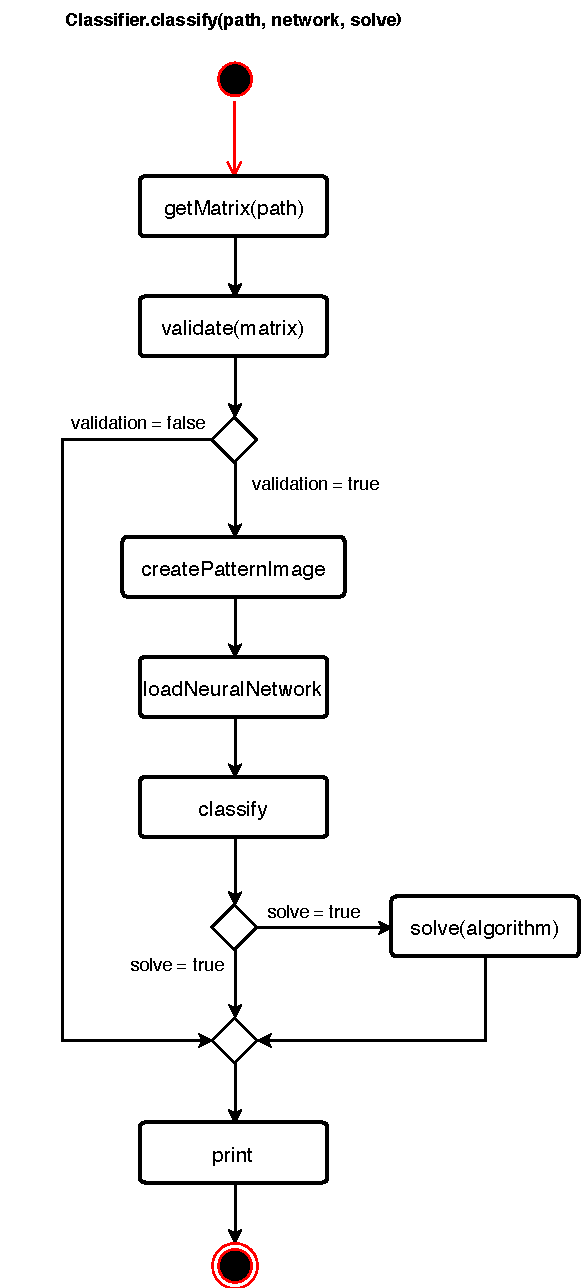
\includepdf[pages={1}]{ActivityDiagrams/PDF/classification}
\label{Activity Diagrams}
\end{center}
\end{figure}

The collector component is responsible for acquiring, creating, collecting and saving matrices into a dataset. It consists of six classes:
the Collector class which is the entry point of the component. The Collector class has one Generator object for generating matrices and one Saver object for saving a dataset. The Generator class has one Validator util class for checking regularity, one Ssget object for fetching and cutting matrices from the SuiteSparse Matrix collection and multiple matrix objects for initializing and returning matrices.

\subsection{Class Description}

\subsubsection{Class Collector}
The Collector class is responsible for collecting a given amount of matrices and saving it into a HDF5 dataset.
When the user types collect into the CLI, a Collector object will be created and the public method collect() with its parameters:
amount, name, size, density and path
will be called. 
The class has a Saver class attribute and a Generator class attribute.
It uses methods from the Generator class to get matrices to collect and methods from the Saver class to save the collected dataset.
(see the collect method Activity Diagram for a more detailed overview).
The Collector class is the interface between matrix collecting and the CLI and conceals all the classes of the Collector described in the following.

\subsubsection{Class Generator}
The Generator class is responsible for actually generating matrices by transforming raw matrices from SuiteSparse and validating them.
The generate(size: Integer, density: Integer):Matrix method is called by a Collector object, uses the Matrix class to initialize an empty matrix, uses the Ssget class to fetch and transform matrices from the SuiteSparse collection and uses the static Validator.validate(matrix: Matrix)  method to check if the matrix is regular and can be returned.

\subsubsection{Class Ssget}
The Ssget class is responsible for fetching matrices from the SuiteSparse collection, transforming them and returning them.
Its getMatrix method is called by a generator object.
The getMatrix method uses the Matrix class to initialize a matrix, then the private downloadMatrix method to fetch a matrix from SuiteSparse, and after that uses its private cutMatrix method to cut a fixed size, regular matrix out of it.

\subsection{Activity Diagrams}
The collect method is executed in the following manner:
\newpage
\begin{figure}[h]
\begin{center}
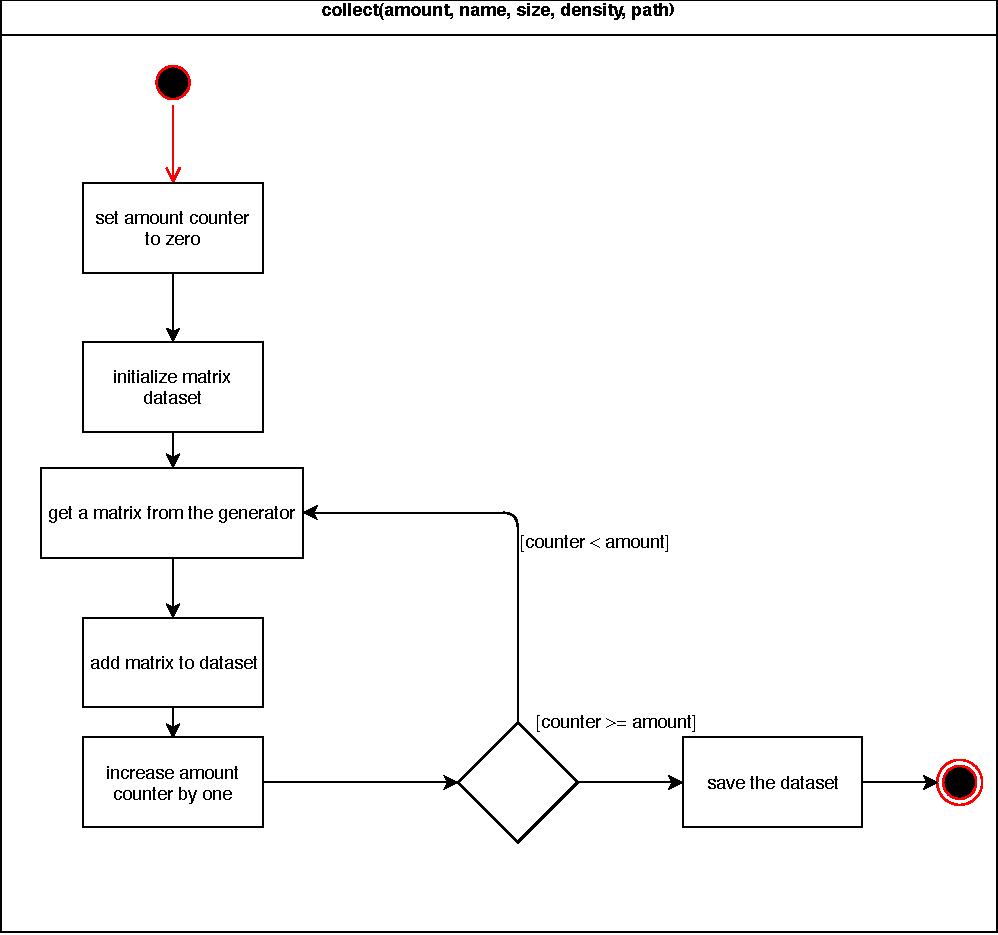
\includepdf[width=\textwidth, height= \textheight, keepaspectratio]{ActivityDiagrams/PDF/Collector_collect_activity.pdf}
\label{Activity Diagrams}
\end{center}
\end{figure}
\newpage


This activity diagram gives a brief overview on how the collector works. First of all a counter is set to zero. Then a matirx dataset for the later collected matrices is initialized. After that a matrix will be fetched from the generator and added to the already initialized dataset.
At last, the counter is increased by one and after that, when the counter equals the amount, the dataset is saved by the saver. If the counter is still smaller than the given amount, another matrix will be fetched. 

\newpage
\begin{figure}[h]
\begin{center}
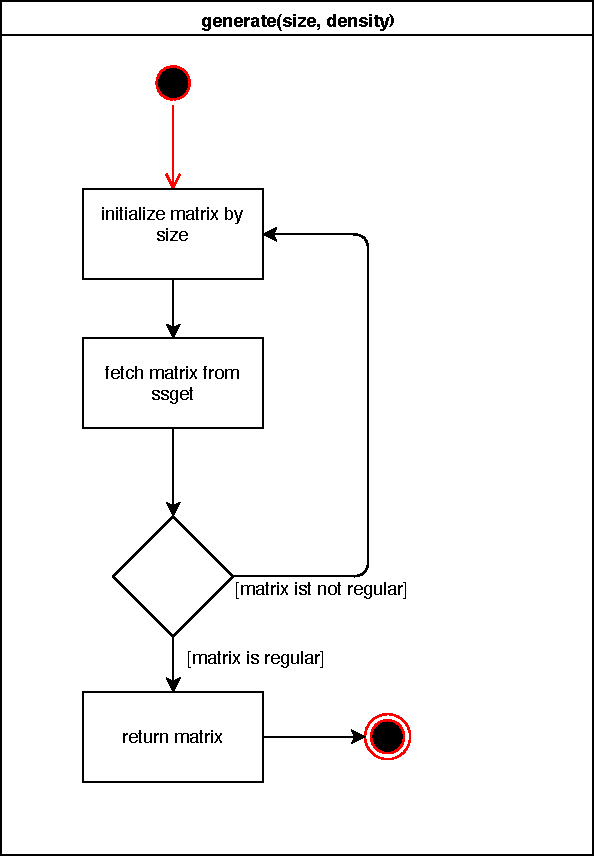
\includepdf[width=\textwidth, height= \textheight, keepaspectratio]{ActivityDiagrams/PDF/Collector_generate_activity.pdf}
\label{Activity Diagrams}
\end{center}
\end{figure}
\newpage

This activity diagram shows are matrices are generated when collecting them to create a dataset. At first an empty matrix with the given size is initialized. After that a matrix is fetched from ssget. When the matrix is regular(this is checked by the Validator) then it will be returned. Otherwise another matrix will be fetched.

\section{Labeling Module}
The labeling module is responsible for the labeling of the sparse matrices. The \gls{label} of a matrix describes which \gls{preconditioner}/\gls{iterative solver} combination solves the given matrix the fastest. The \gls{label} is represented by a vector. Each entry in the vector corresponds to one \gls{preconditioner}/\gls{iterative solver} combination. The entry of the fastest one is 1, all other entries are zero. The matrices with the corresponding \glspl{label} will be used to train the neural network in the training module.

\newpage
\begin{figure}[h]
\begin{center}
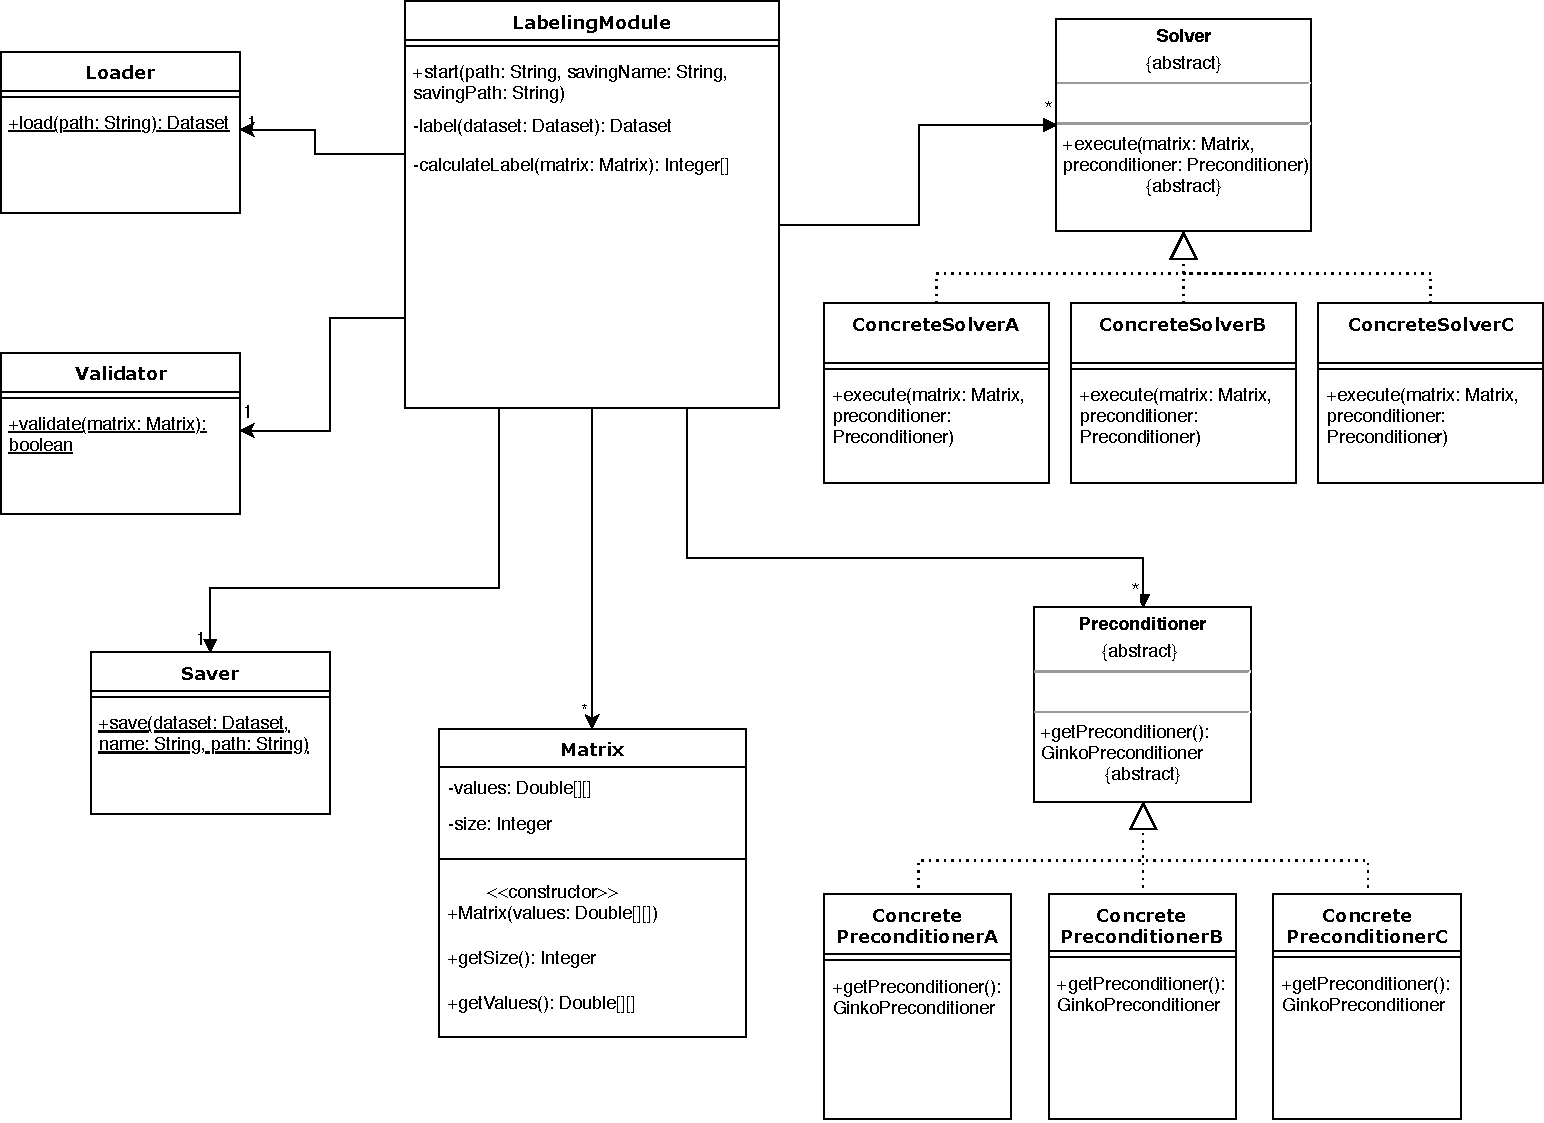
\includepdf[width=\textwidth, height= \textheight, keepaspectratio]{ClassDiagrams/PDF/LabelingModule_classdiagram.pdf}
\label{Labeling Module}
\end{center}
\end{figure}
\newpage

The main component of the labeling module is the class labeling module. It provides the only public method in the labling module, the method start(path:String, savingName:String,savingPath:String). This method is the entry point of the module and will start the labeling process of the provided matrices(specified by the path). \newline\newline

The class labeling modue has a set of matrices which the module will label.\newline\newline

The module furthermore has a Loader class. The class labeling module has exactly one Loader class. This class is responsible for loading the matrices which get labeled. Its only method is the method load(path:String) which gets a path of a hdf5 file supplied and returns a dataset. If the specified path is not a hdf5 file, the programm will print an error to the command line. \newline\newline

Another class in the labeling module is the Saver class. The class labeling module has exactly one Saver class. This class is responsible for the saving of the matrices and the \glspl{label}. Its only method is the method save(dataset:Dataset,path:String). If this method is called, the specified dataset will be safed at the specified path. The matrices and the \glspl{label} will be safed in one hdf5 file.\newline
\newline
The labeling module class moreover has a validator class. This class is responsible for determining wheter the given matrix is regular. If that is not the case, the matrix will be deleted.
\newline\newline
Since the labeling module is responsible for finding the best \gls{preconditioner}/\gls{iterative solver} combination for a given set of matrices, the module furthermore has a \gls{preconditioner} and a Solver class. Those classes are abstract. ConcreteSolvers inherit from the class Solver and Concrete\gls{preconditioner}s from the class \gls{preconditioner}.\newline\newline

The Solver class contains the logic for solving a matrix with an \gls{iterative solver}. Each ConcreteSolver corresponds to one \gls{iterative solver}.Each class of ConcreteSolver has the method execute(Matrix,\gls{preconditioner}) which will solve a given matrix. We will be using the design pattern "stragety" for the \gls{iterative solver}s. The reason being that each Solver does basically the same thing(solving a matrix) in a different manner. The user moreover has no influence on which Solver we will be using at any given time.
Each Solver will take an optional precondtioner as its input for the method execute(Matrix,\gls{preconditioner}). The \gls{preconditioner} will be used at every step of the \gls{iterative solver}. We will be using the design pattern "\gls{strategy}" for the \gls{preconditioner}s too. \gls{preconditioner}s each return a Ginko\gls{preconditioner} which will be used by the Solver class to communicate with the ginkgo libary. So each Concrete\gls{preconditioner} basically does the same thing(returning a \gls{preconditioner}). The user furthermore has no influence on which \gls{preconditioner} we will be using at any given time. That is why the "\gls{strategy}" design pattern is applicable.

\subsection{Class Descriptions}

\subsubsection{Class LabelingModule}
The class LabelingModule is the main component of the labeling module. It provides one public method start(path:String, savingName:String,savingPath:String) which is the entry point for the labeling module. When the user types label in the command line this command will be executed. The arguments of the start method are optional. If there are no arguments provided the labeling module will be using default paths. The default paths are specified in a configuration file(see the training module for further details). If the User specifes his own paths they have to be vaild. Valid in this case means that the path points to a hdf5 file with the correct formatation. If this is not the case the program will print an error message to the command line and execute a controlled shutdown so that the user can specify a correct path.
\subsubsection{Class Solver}
An Solver in our sense is an interative Solver which is able to to solve a linear system Ax=b for x, where A is a (in our case sparse) matrix of size nxn, x is a vector of size 1xn and b is vector of size 1xn(n$\in$N). The matrix A in our case will be the Matrix the method execute(matrix,preconditioner) will receive, the vector b will be a random vector with values between 0 and 1. We chose the vector to be random since the choice of b has no great influence on the time it takes to solve the linear system.
%find correct symbol for N
The \gls{iterative solver} uses an iterative approach to solve the linear sysetm. An iterative approach is characterized by the idea that the linear system gets solved step by step, where the solution of one step enables the solution of the next step. The class \gls{iterative solver} achieves this by communicating with the ginkgo libary, which has an implementation of the solvers. An \gls{iterative solver} may optionally use a \gls{preconditioner} for its calculation. Since there are many different \gls{iterative solver}s which achieve the same outcome(solving for x) we will be using the design pattern "\gls{strategy}". That is why the class Algortihm is abstract and ConcreteSolvers (which actually represent one \gls{iterative solver} each) will inherit from Solver. The user at no point decides which Solver gets used at any given time. \newline
A Solver has one method execute(Matrix,\gls{preconditioner}) ,which takes a matrix (and a \gls{preconditioner}) and solves it. The time the \gls{iterative solver} takes to solve the matrix will be recorded and in the class labelingModule used to label the matrix. All ConcreteSolvers have to implement the abstract function execute.

\subsubsection{Class ConcreteSolver}
A ConcreteSolver is the actual representation of one \gls{iterative solver}.

\subsubsection{Class \gls{preconditioner}}
A \gls{preconditioner} is a transformation of a linear system Ax=b for x, where A is a (in our case sparse) matrix of size nxn, x is a vector of size 1xn and b is vector of size 1xn(n$\in$N). A transformation may be a Matrix p (nxn) which would result in the linear system PAx = Pb. A \gls{preconditioner} is used so that the linear system may be solved more easily by an \gls{iterative solver}. The transformation of the \gls{preconditioner} is applied in every step of an \gls{iterative solver}. \newline\newline
The class \gls{preconditioner} only has one method, get\gls{preconditioner}() which will return the Ginko\gls{preconditioner} corresponding to the \gls{preconditioner} class. The \gls{preconditioner} class achieves this by communicating with the ginkgo libary.

\subsubsection{Class Concrete\gls{preconditioner}}
A Concrete\gls{preconditioner} is the actual representation of one \gls{preconditioner}.

\newpage
\subsection{Activity Diagrams}
When the user types label() in the CLI the moethod start() in the class LabelingModule will be executed in the following manner:

\begin{figure}[h]
\begin{center}
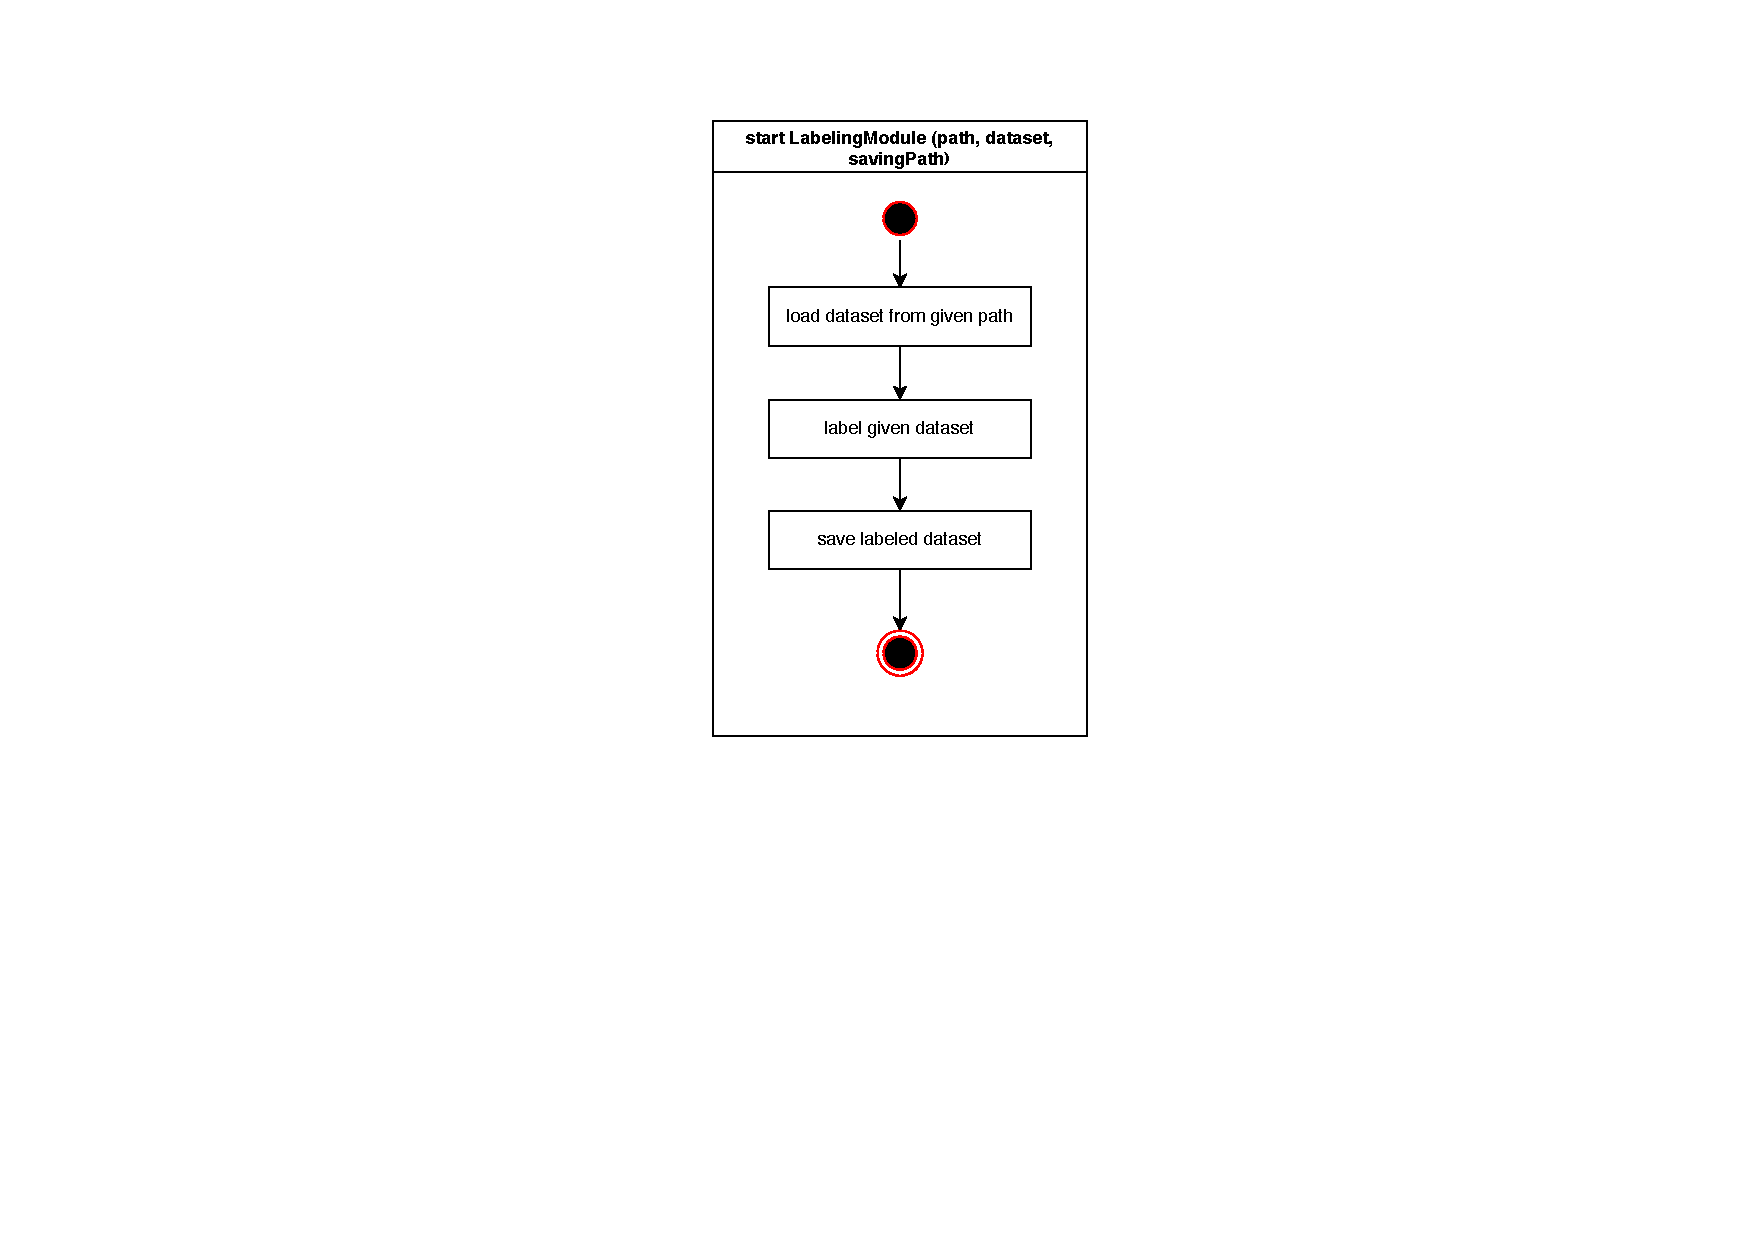
\includepdf[width=\textwidth, height= 15cm, keepaspectratio]{ActivityDiagrams/PDF/LabelingModule_start_activity.pdf}
\label{Activity Diagrams}
\end{center}
\end{figure}
\newpage


The activity diagram ``start LabelingModule'' shows the general overview of what the LabelingModule does.The shown method start() is the only public method in the LabelingModule class, therefore the only way to communicate whit it.
First of all the dataset to work on will be loaded from the given path, which contains all matrices the LabelingModule has to label.
After that the dataset will be labeled (explained in detail in the ``label given dataset'' activity diagram).
Last but not least the new dataset with \glspl{label} will be saved under the given savingPath.


\begin{figure}[h]
\begin{center}
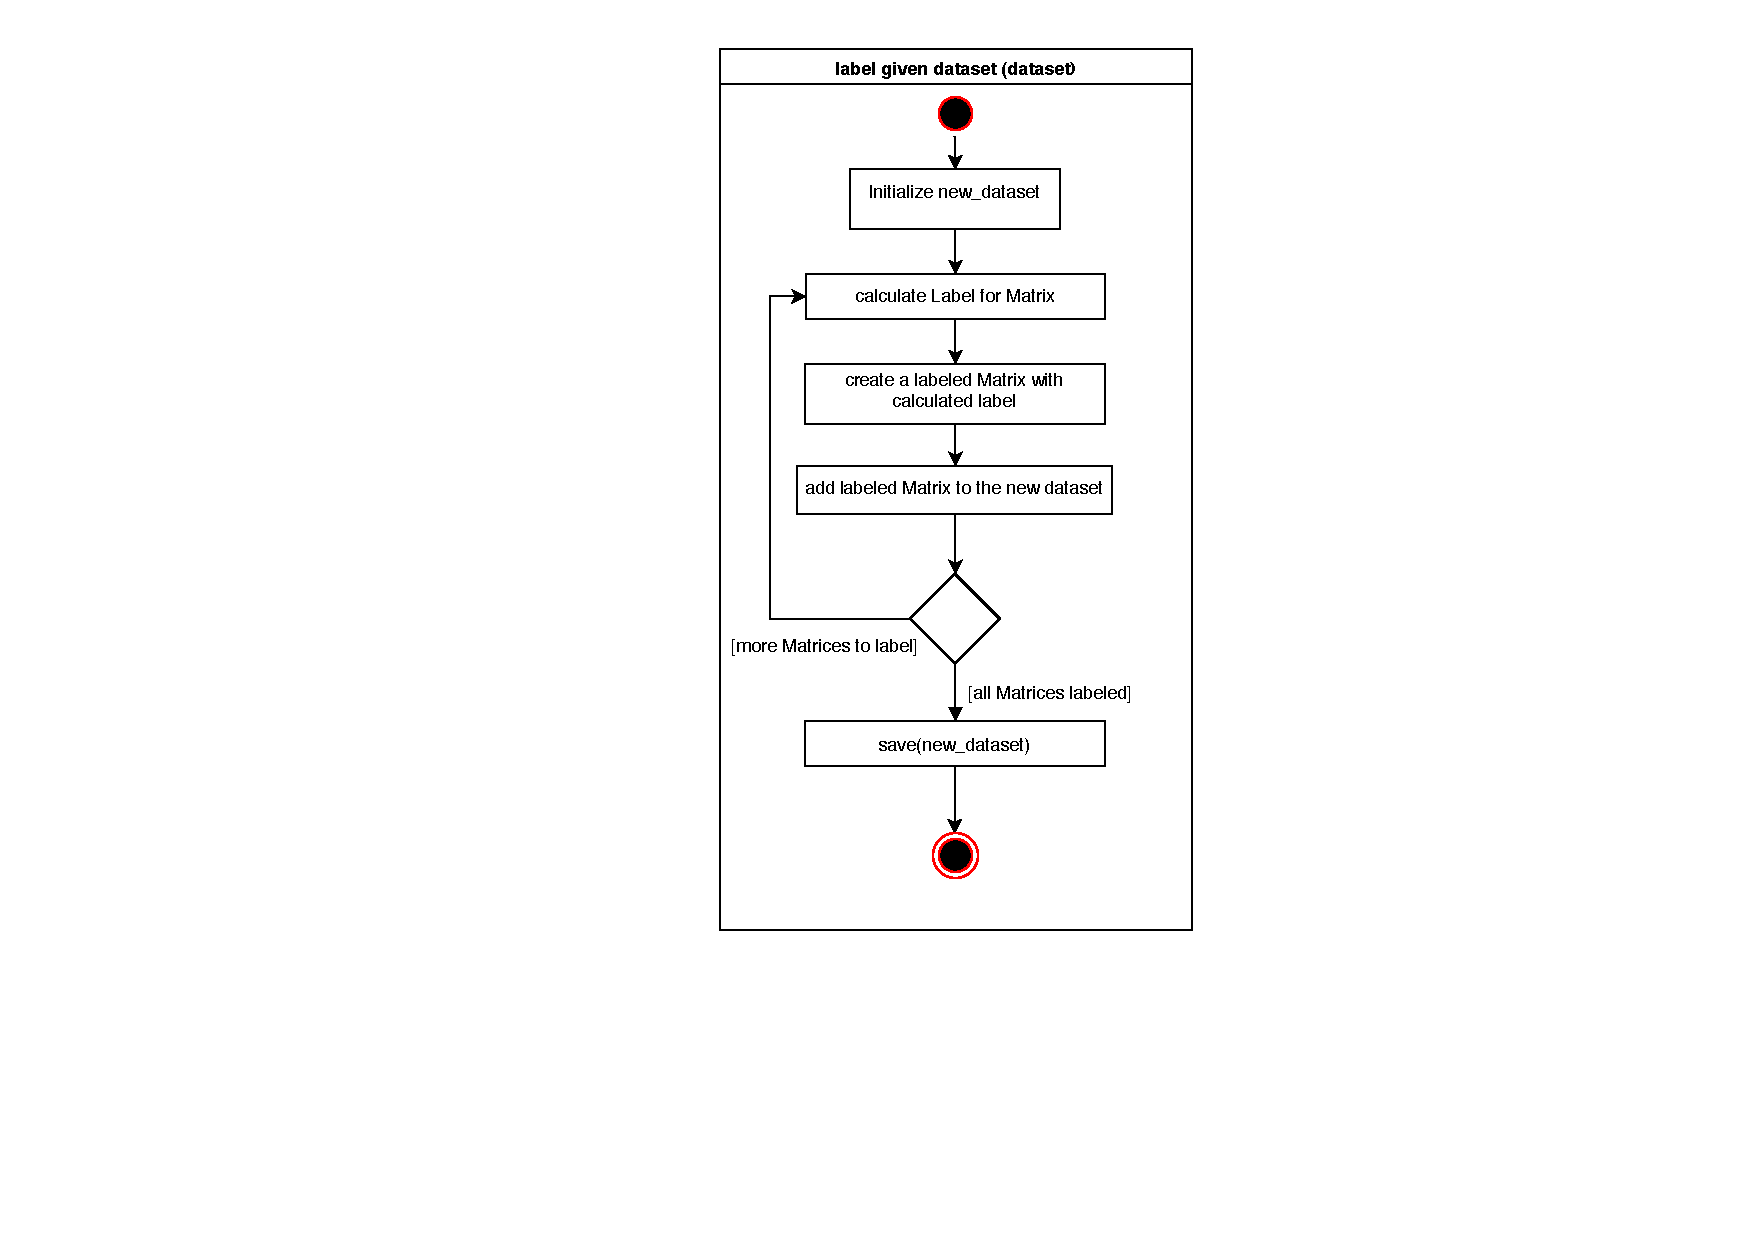
\includepdf[width=\textwidth, height= 15cm, keepaspectratio]{ActivityDiagrams/PDF/LabelingModule_label_activity.pdf}
\label{Activity Diagrams}
\end{center}
\end{figure}
\newpage


The activity diagram ``label given dataset'' shows how the class LabelingModule labels a dataset.First of all a new dataset is initialized.
The following steps will be made on each matrix in the dataset.
First of all the matrix is validated, to see whether the matrix is regular or not, if the matrix isn't regular the matrix will be removed. In case that the matrix is regular, the \gls{label} for the matrix is calculated (explained in the ``calculate label for given matrix activity diagram'').  The calculated \gls{label} will be saved in the new dataset.
As soon as every matrix has been labeled the new dataset is returned.


\newpage
\begin{figure}[h]
\begin{center}
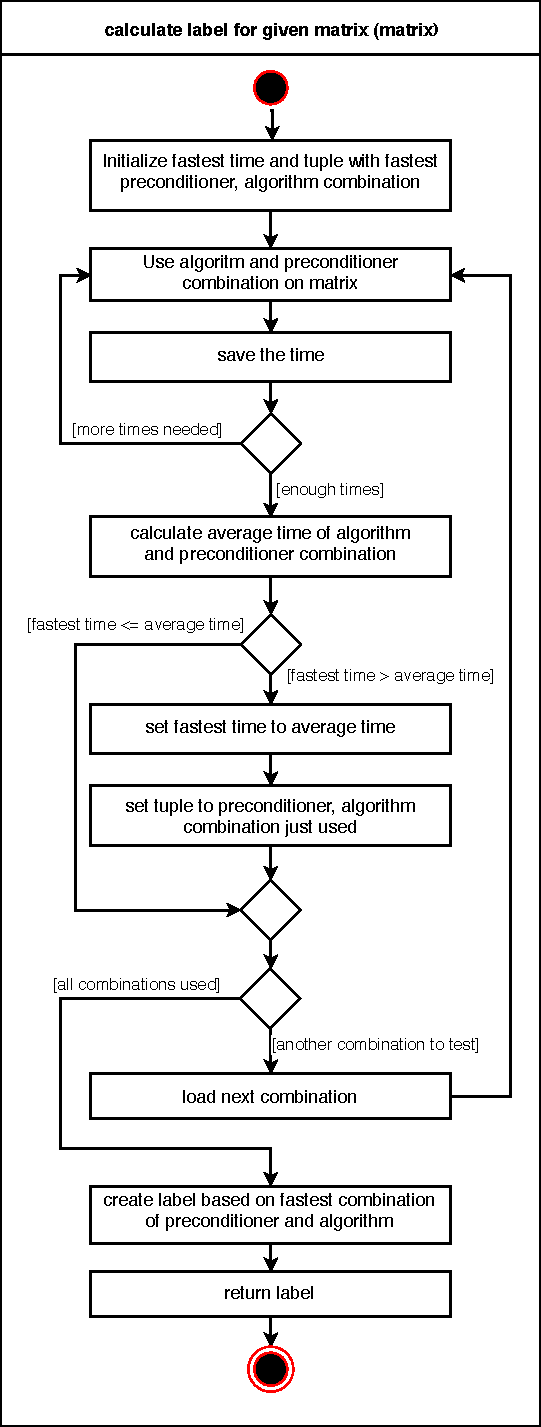
\includepdf[width=\textwidth, height= \textheight, keepaspectratio]{ActivityDiagrams/PDF/LabelingModule_calculateLabel_activity.pdf}
\label{Activity Diagrams}
\end{center}
\end{figure}
\newpage

The activity diagram ``calculate label for given matrix'' shows how a \gls{label} is calculated for a single matrix. First of all a fastest item variable and a \gls{tupel} of \gls{preconditioner},\gls{iterative solver} is initialized.
The first \gls{preconditioner},\gls{iterative solver} combination is used on the matrix and the time it took to solve given matrix is saved, that process is looped, until we have enough saved time data.
Out of the saved times for the \gls{preconditioner},\gls{iterative solver} combination the average time the combination took will be calculated. The calculated average time will be written in the fastest time variable and the combination in the \gls{tupel} previously initialized. After that a new combination is loaded, if there is another one to test.
For each new combination the process of using the combination, saving the time and calculating the average time remains the same. After the average time of the new combination is calculated. After that there are two options. 1. if the average time of the new combination is smaller than the time saved in the fastest time variable, the fastest time variable gets overwritten with the new average time and the new combination is also getting written in the \gls{tupel}.2. the fastest time is smaller then the new average time, is that the case, the new average time and combination is ignored.
Last but not least, if all combinations are finished testing a \gls{label} is created based on the current fastest time and \gls{preconditioner}, \gls{iterative solver} combination and the \gls{label} is returned.

\subsection{Sequence Diagrams}
The sequence diagram shows what happens when the start() method of the LabelingModule is called. First of all the method load(), with the parameter path, of the Loader class is called,the path is either the path the user wrote in his input, or it is the standard path, which is specified in the Configuartion Fil. The load() method returns the dataset the LabelingModule will be working on. After that, the LabelingModule calls its own method label() with the just received dataset. The label() method then goes into a loop, covering each matrix on its own.
For each matrix, the validate() method of the Validator gets called with the parameter matrix. validate() returns a boolean, whether the matrix is regular (true) or not (false).
If the matrix is regular, the method calculate\_label() of the LabelingModule with the parameter matrix is called. calculate\_label returns a \gls{label}. if the matrix isn't regular, or the \gls{label} is calculated the loop starts with the next matrix, until there are none left.After all \glspl{label} are calculated they all are summarized in a dataset.
The new dataset is after that one of the parameters for the save() method of the Saver class, which saves the new dataset, with the given namen in the given path.

\newpage
\begin{figure}[h]
\begin{center}
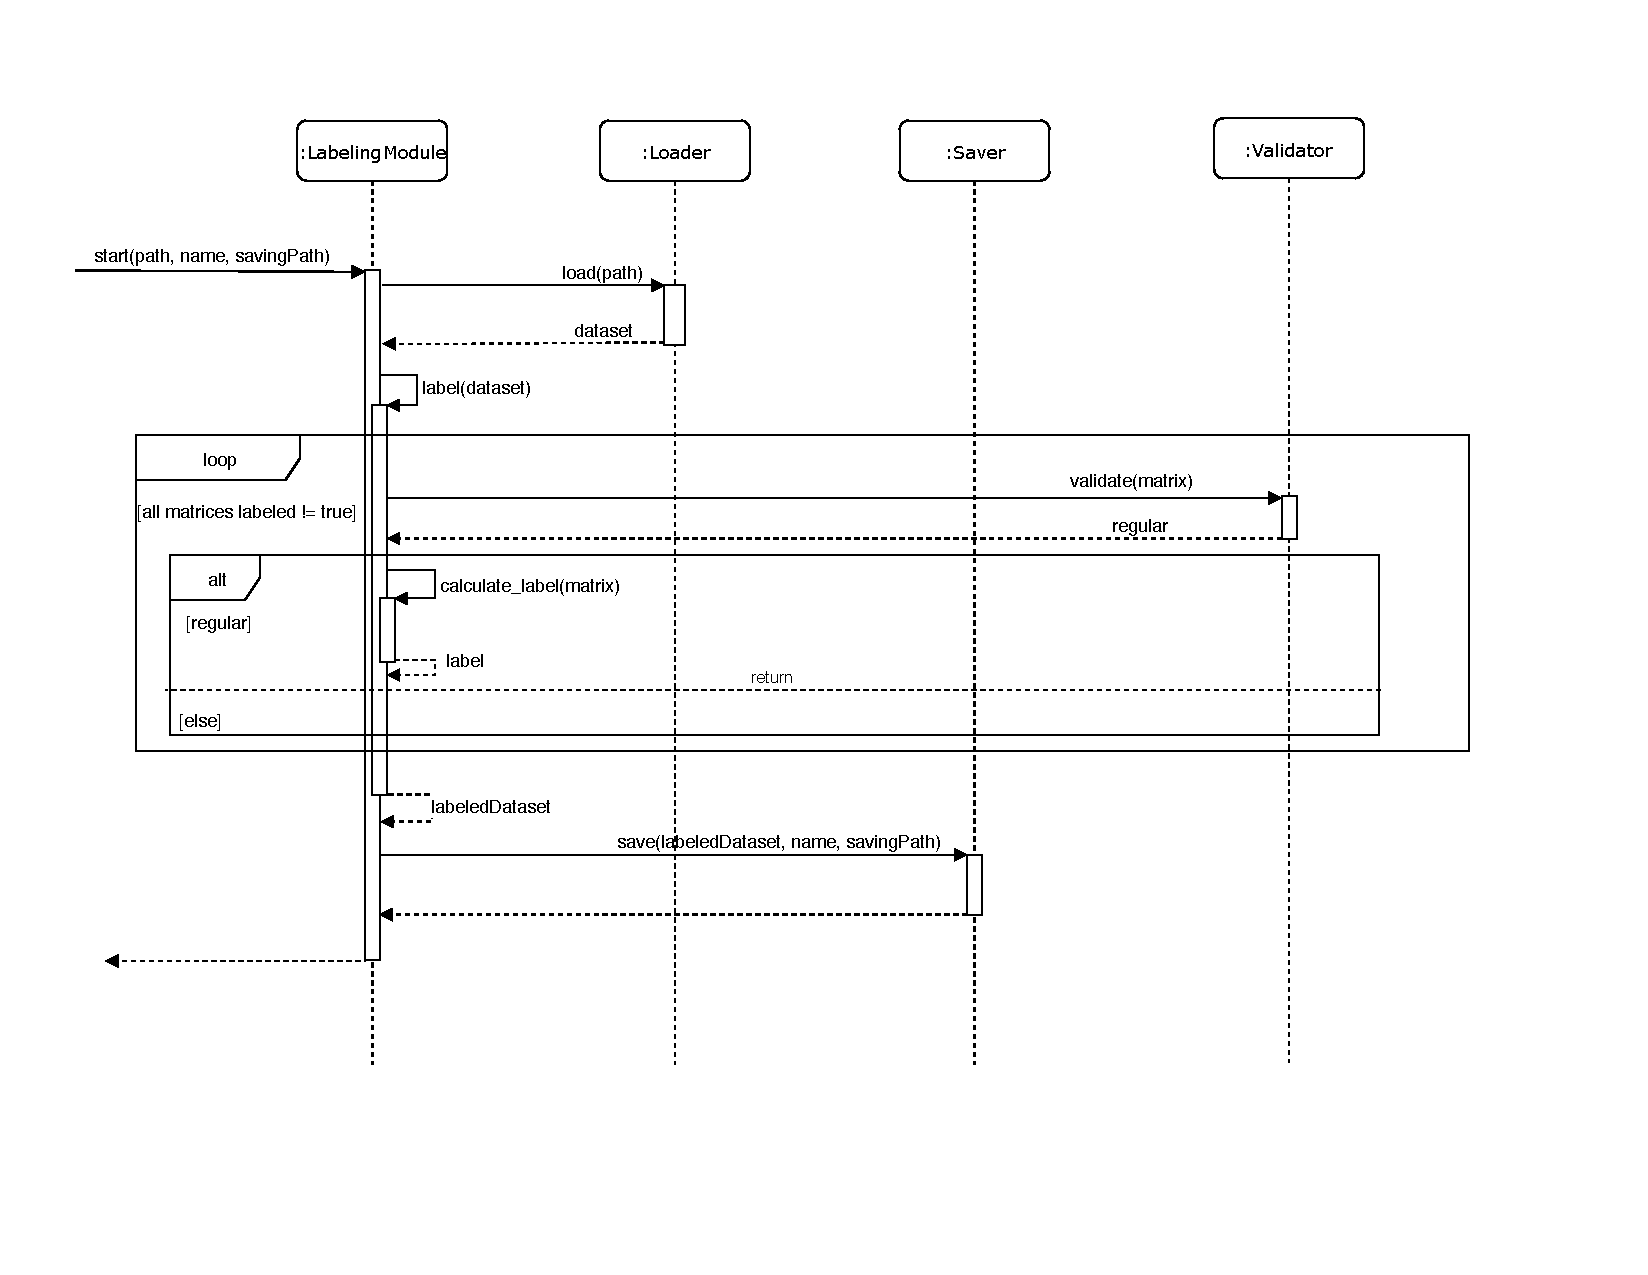
\includepdf[width=\textwidth, height= \textheight, keepaspectratio]{SequenceDiagram/PDF/LabelingModule_start_sequenzdiagram.pdf}
\label{Activity Diagrams}
\end{center}
\end{figure}
\newpage



\section{Training module}
The training module is responsible for the training and testing of a neural network. It is structured in 2 parts, the configuration file and the class training module. The class training module loads its configuration from the configuartion file. It furthermore uses a set of labled matrices for the training and testing. With the configuration set, the class training module will start the training and testing. The trained network will be saved to a specified path.
%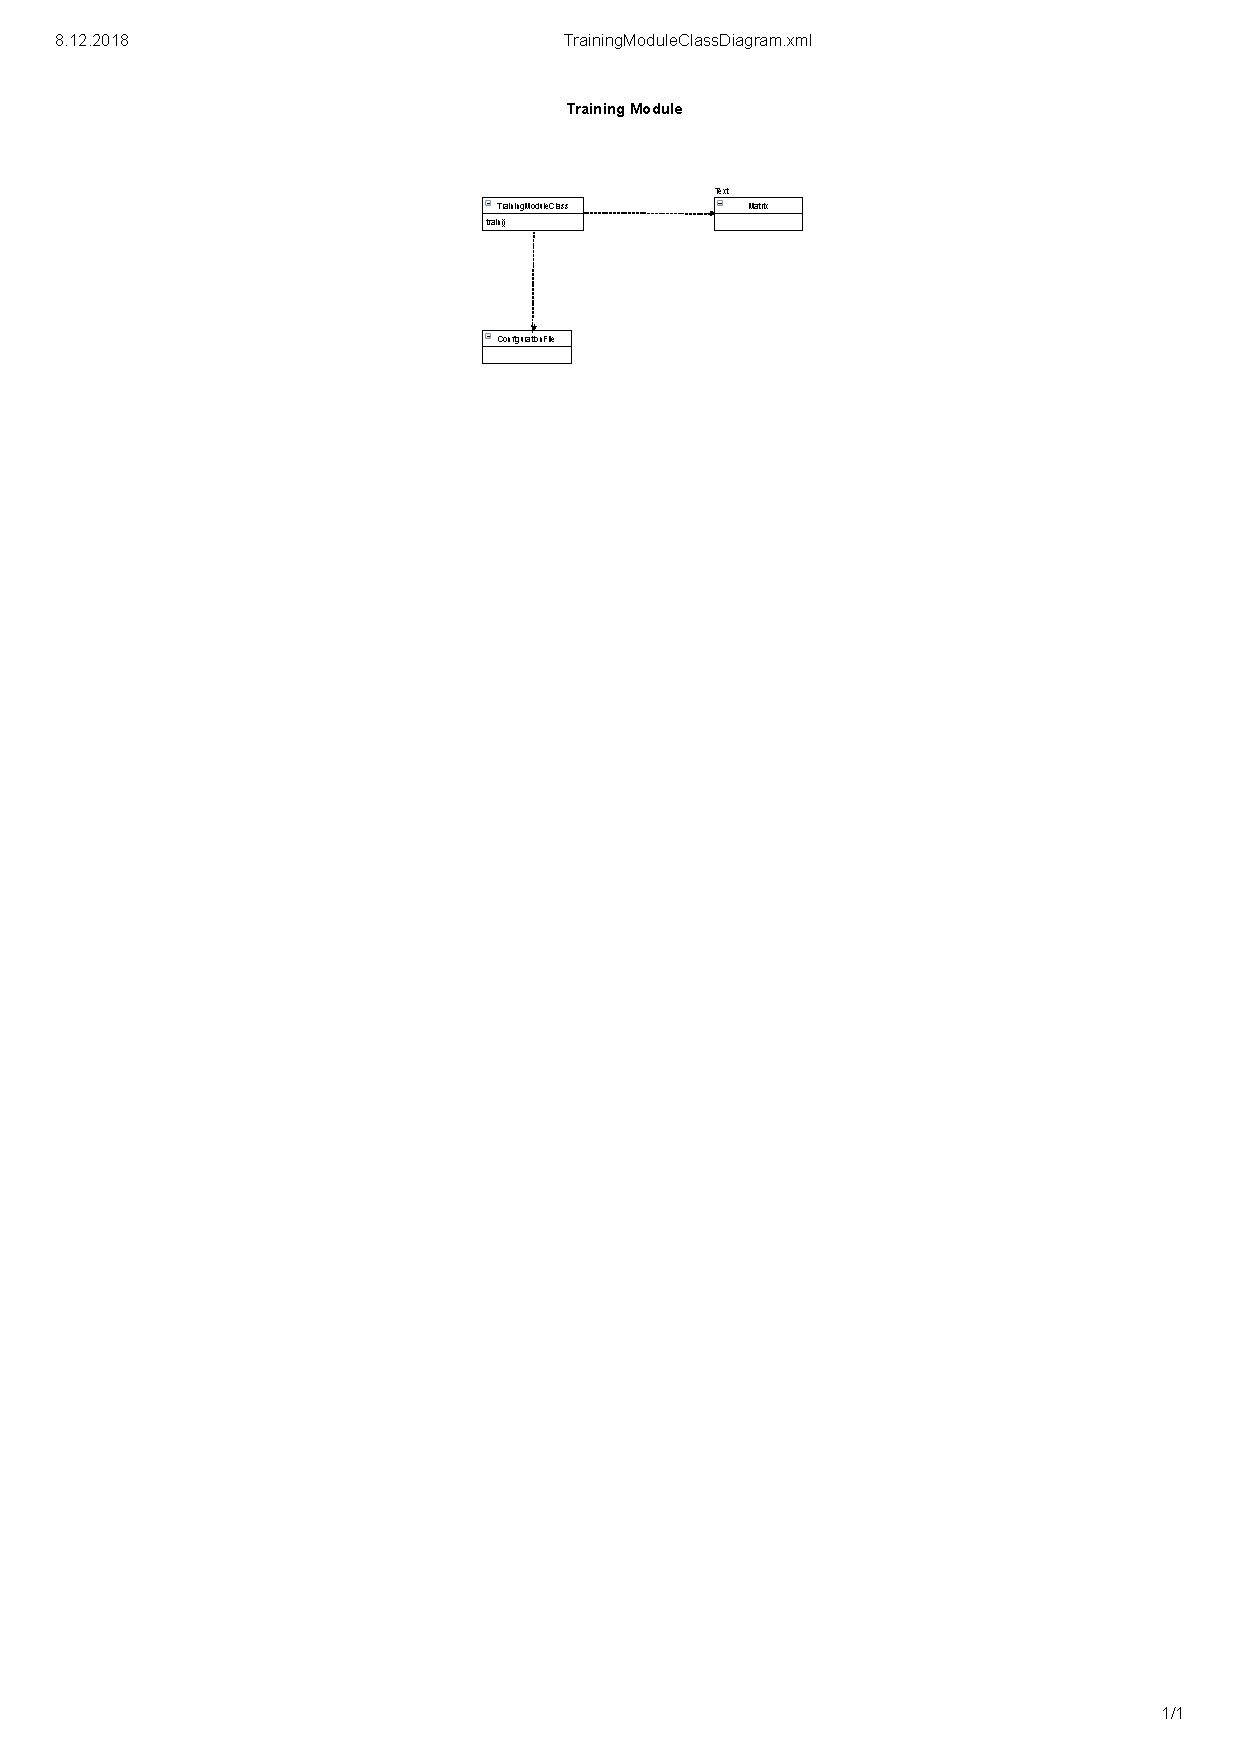
\includepdf[pages={1}]{ClassDiagrams/PDF/TrainingModuleClassDiagram}
\begin{figure}[h]
\begin{center}
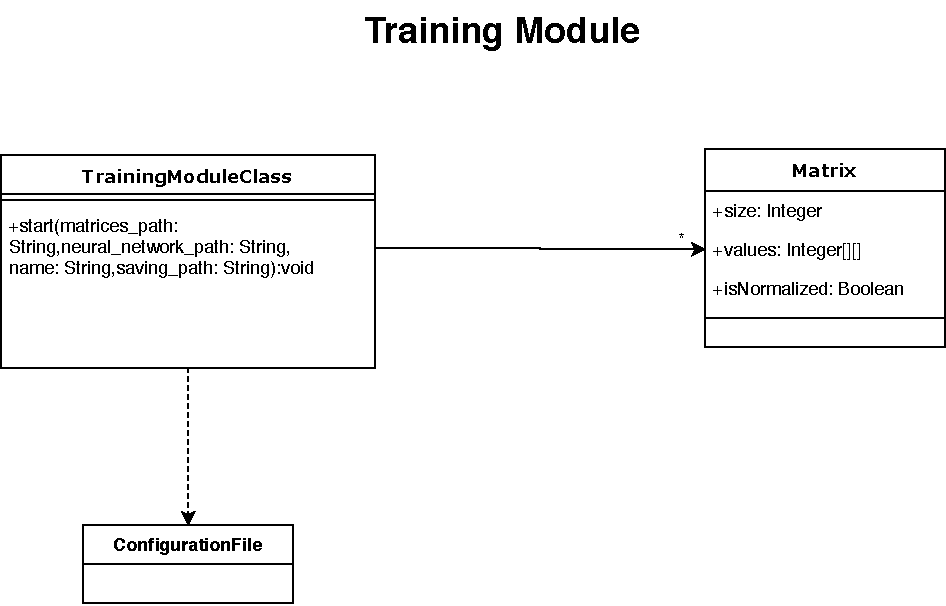
\includegraphics{ClassDiagrams/PDF/TrainingModule_classdiagram.pdf}
\label{Activity Diagrams}
\end{center}
\end{figure}

%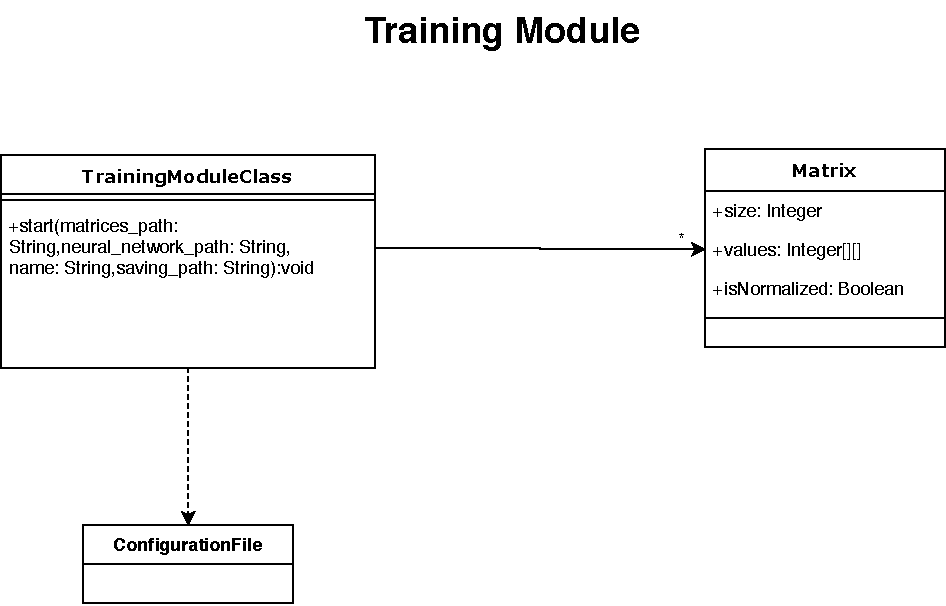
\includegraphics{ClassDiagrams/PDF/TrainingModule_classdiagram.pdf}
\subsection{Class descriptions}
\subsubsection{Class Configuration File}
The configuration file is a text file. The information will be loaded with a configuration file parser.
It is used to specify all necessary information the class neural network needs to train the neural network.
If the user does not change anything in the configuration file, defaut options for the model definiton and hyperparameters will be used. The loading and saving paths may be changed via the command line. The configuration file is organized in four main categories.
\begin{enumerate}
\item default loading path of the set of matrices 
\item default saving path for the neural network
\item default loading path for the neural network
\item default model definition and hyperparameters
\end{enumerate}
The loading path of the set of matrices is the path in which the matrices that are used for the training and testing are stored.
The training module only supports one hdf5 file.
If the path is any other file, the labling module will print an error message to the command line so that the user can specify a valid path.
For the training and testing making sense there should be at least 500 matrices in the hdf5 file.
Otherwise the accuracy of the neural network will be so low that i can not be used for classification.
If there is no path specified in the start method, the training module will use a default path.
In the default path will be the latest matrices that the labling module has produced. \newline

The saving path for the neural network is the path where the trained and tested neural network will be safed.
It will be safed as a Keras model.
If there is no path specified in the start method, the neural network will be safed at a default destination.
If there is no path for the neural network specified in the module Classifier the module will use this default path to load its neural network.\newline

The loading path for the neural network is strictly optional.
If this path is specified in the method start the training module will use the neural network in the path for training and testing.
This option enables the user to use a pre-trained neural network for training.
This could be the case if the user interrupts the training process at a certain time and wants to to repeat the training later.
Other use cases are of course possible too.
The neural network has to be a model of the Keras framework. If the path is any other file the training module will print an error so that the user can specify a valid path.
If this path is not specified the training module will create a new neural network(with the model definition and hyperparamters of the next category) and train with it. \newline

The model definition and hyperparameters are used to determine which neural network will be trained and tested. The model definition determines the following:
\begin{itemize}
\item the amount of layers
\item the amount of nodes in every layer
\item the kind of neural network(e.g. Convolutional)
\item the activation function
\item the regularization
\item the optimizer
\end{itemize}

The hyperparamters determine the following:

\begin{itemize}
\item the dropout
\item the batch size
\item how much of the data should be training and how much should be testing data
\item the network weight initialization
\item the learning rate
\end{itemize}

\subsubsection{Class TrainingModule}
The TrainingModule class is responsible for the training and testing of a neural network.
It can not be instantiated, since it is a utility class.The structure is mainly oriented towards the keras workflow and will be further described later in the activity diagramm.
The class offers one public method, the method start(matrices\_path: String,neural\_network\_path: String,
name: String,saving\_path: String). \newline

We will furthermore be using the function keras.callbacks.ModelCheckpoint to save the neural network after every epoch. This will guarantee that we do not loose all training progress if the computer crashes or other unexpected events happen. The proceedure is consitent with the design pattern \gls{memento}.


\subsection{Activity Diagarams}
When the user types train in the CLI the method train in the class TrainingModule will be executed in the following manner:

\begin{figure}[h]
\begin{center}
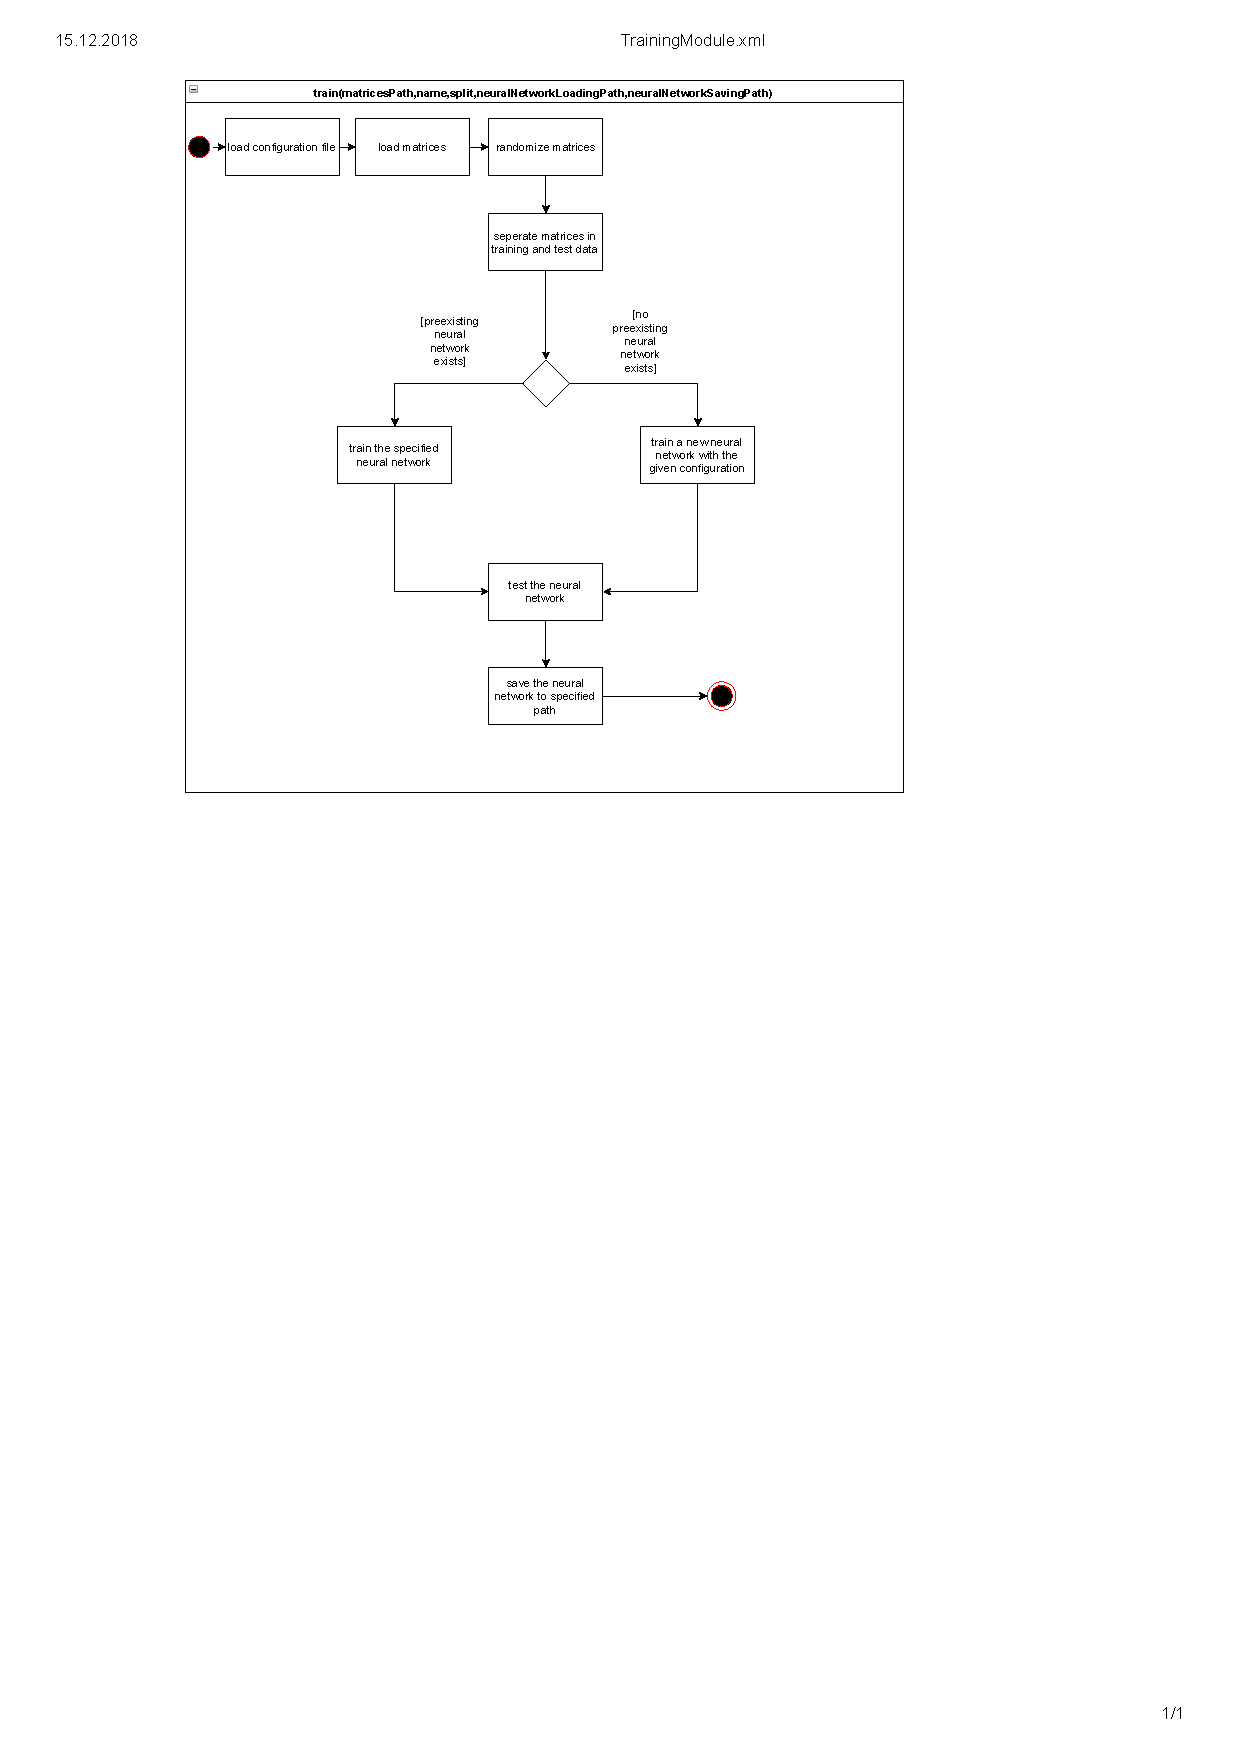
\includegraphics[scale=0.9]{ActivityDiagrams/PDF/TrainingModule}
\label{Activity Diagrams}
\end{center}
\end{figure}

\begin{itemize}
\item load the configuration file
\item load the labeled matrices
\item normalize values of the matrix(between 0 and 1)
\item seperate the labeled matrices in training and test data
\item train a preexisting neural network or a new one(depending on the specifed paths)
\item test the neural network
\item save the neural network
\end{itemize}

The configuration file that gets loaded will be used to specify the subsequent points.\newline

The configuration file will determine from which path the labeled matrices will be loaded.
If there is no path specified in the method start, the default path will be used(see the class description of the configuration file).
The labeled matrices will be loaded in one hdf5 file. If the path links to any other file, the class TrainingModule will print an error to the command line so that the user can specify a valid path. \newline

Then the values of the matrix will be normalized. This means that every entry will be converted to a value between 0 and 1, such that relative distances are kept. This is done because those values will be fed in the neural network and there should not be outliers which result in the neural network not beeing trained properly.

After that the class TrainingModule will seperate the training and test data.
How the data will be seperated is specified in the configuration file.\newline

Following there are two alternatives
 If the user has specified a neural network loading path in the method start, the class TrainingModule will train this neural network with the labeled matrices for the training.
If the user has not specified a neural network  loading path in the method start, the class TrainingModule will create a new neural network with the specifications in the configuration file.\newline

If there are no model definitions in the configuration file the class TrainingModule will use the \gls{default neural network}.
The class TrainingModule then proceeds with training the new neural network with the labeled matrices for the training. In both cases the current loss will be continously printed to the command line.\newline

Now the neural network is trained. The class TrainingModule proceeds with testing the neural network with the labeled matrices for the testing.
This process will determine the accuracy of the neural network on the given test matrices.
The accuracy will be printed on the command line.\newline

After that the neural network will be safed as a keras model.
The path for the saving is specified in the configuration file or by the method start.


\newpage
\section{Classifier}

\subsection{Diagrams}

\subsection{Class Diagrams}

\begin{figure}[h]
\begin{center}
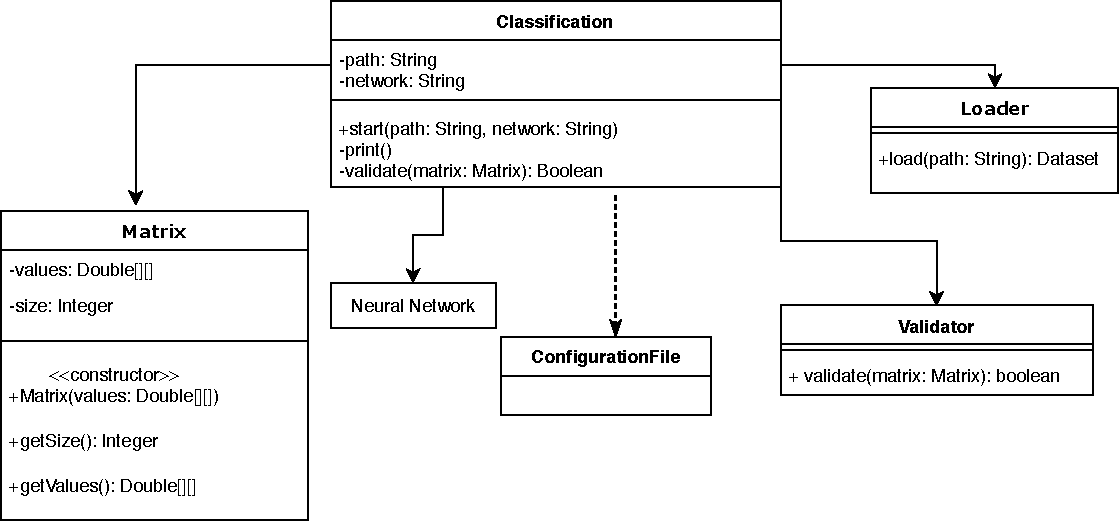
\includepdf[width=\textwidth]{ClassDiagrams/PDF/Classifier}
\label{Class Diagram}
\end{center}
\end{figure}

\newpage


\subsection{Class Descriptions}

\subsubsection{Class Classifier}
The classifier classifies a matrix given by a path. 
In this path, the matrix is stored in the form of an HDF5 file.
As a second parameter the neural network path will be given. 
In this path the trained network the user wants to use for his classification is saved.

\newpage
 
\subsection{Activity Diagrams}

\begin{figure}[h]
\begin{center}
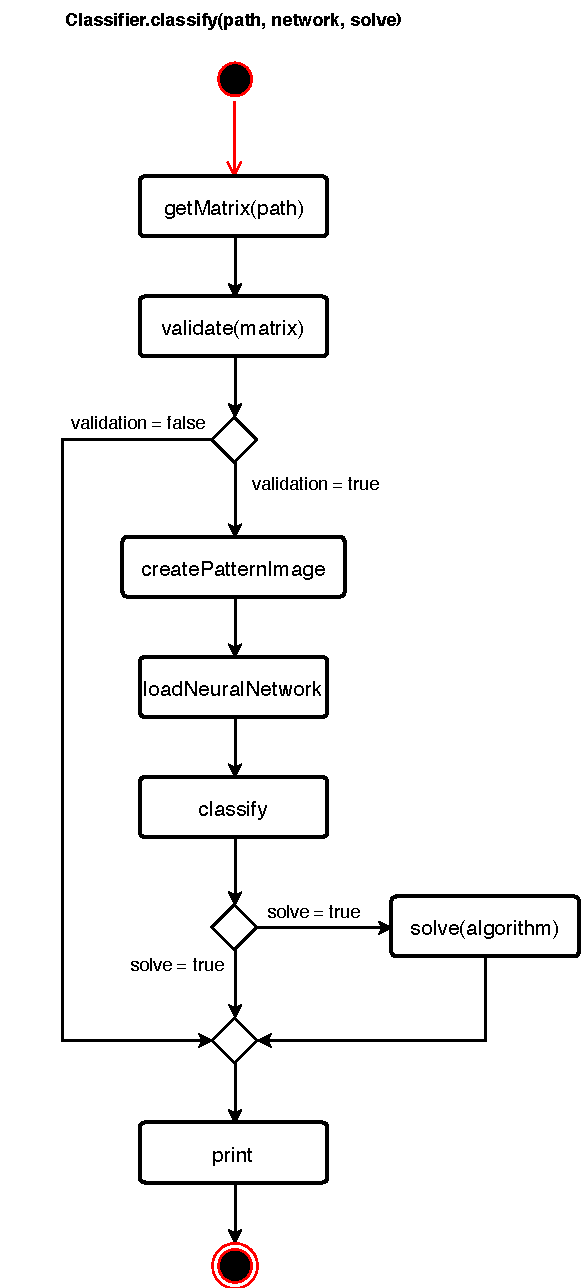
\includegraphics[width=8cm,height=15cm,keepaspectratio]{ActivityDiagrams/PDF/classification}
%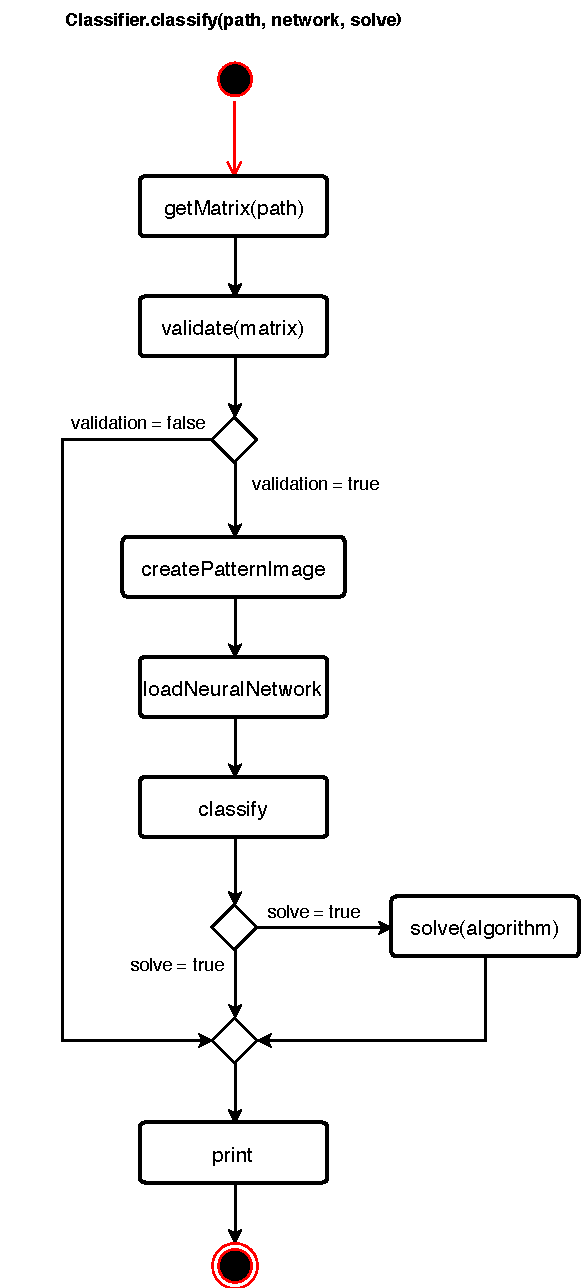
\includegraphics[height=\textheight]{ActivityDiagrams/PDF/classification}
\label{Activity Diagrams}
\end{center}
\end{figure}

\newpage
\subsubsection{Description}
The method start in the class classifier classifies a given Matrix.
First of all the classifier has to get the matrix. 
After that the matrix has to be validated.
This validation will give a boolean back, whether the matrix is regular (true) or not (false).
If the validation is true (validation = true) the matrix will be normalized.
After that the neural network will be loaded, with which in the following the matrix will be classified.
In the last step a result will be printed whether it is the result of the classification or an Error-statement, because the validation was false.

 
\newpage
\subsection{Sequence Diagrams} 

\begin{figure}[h]
\begin{center}
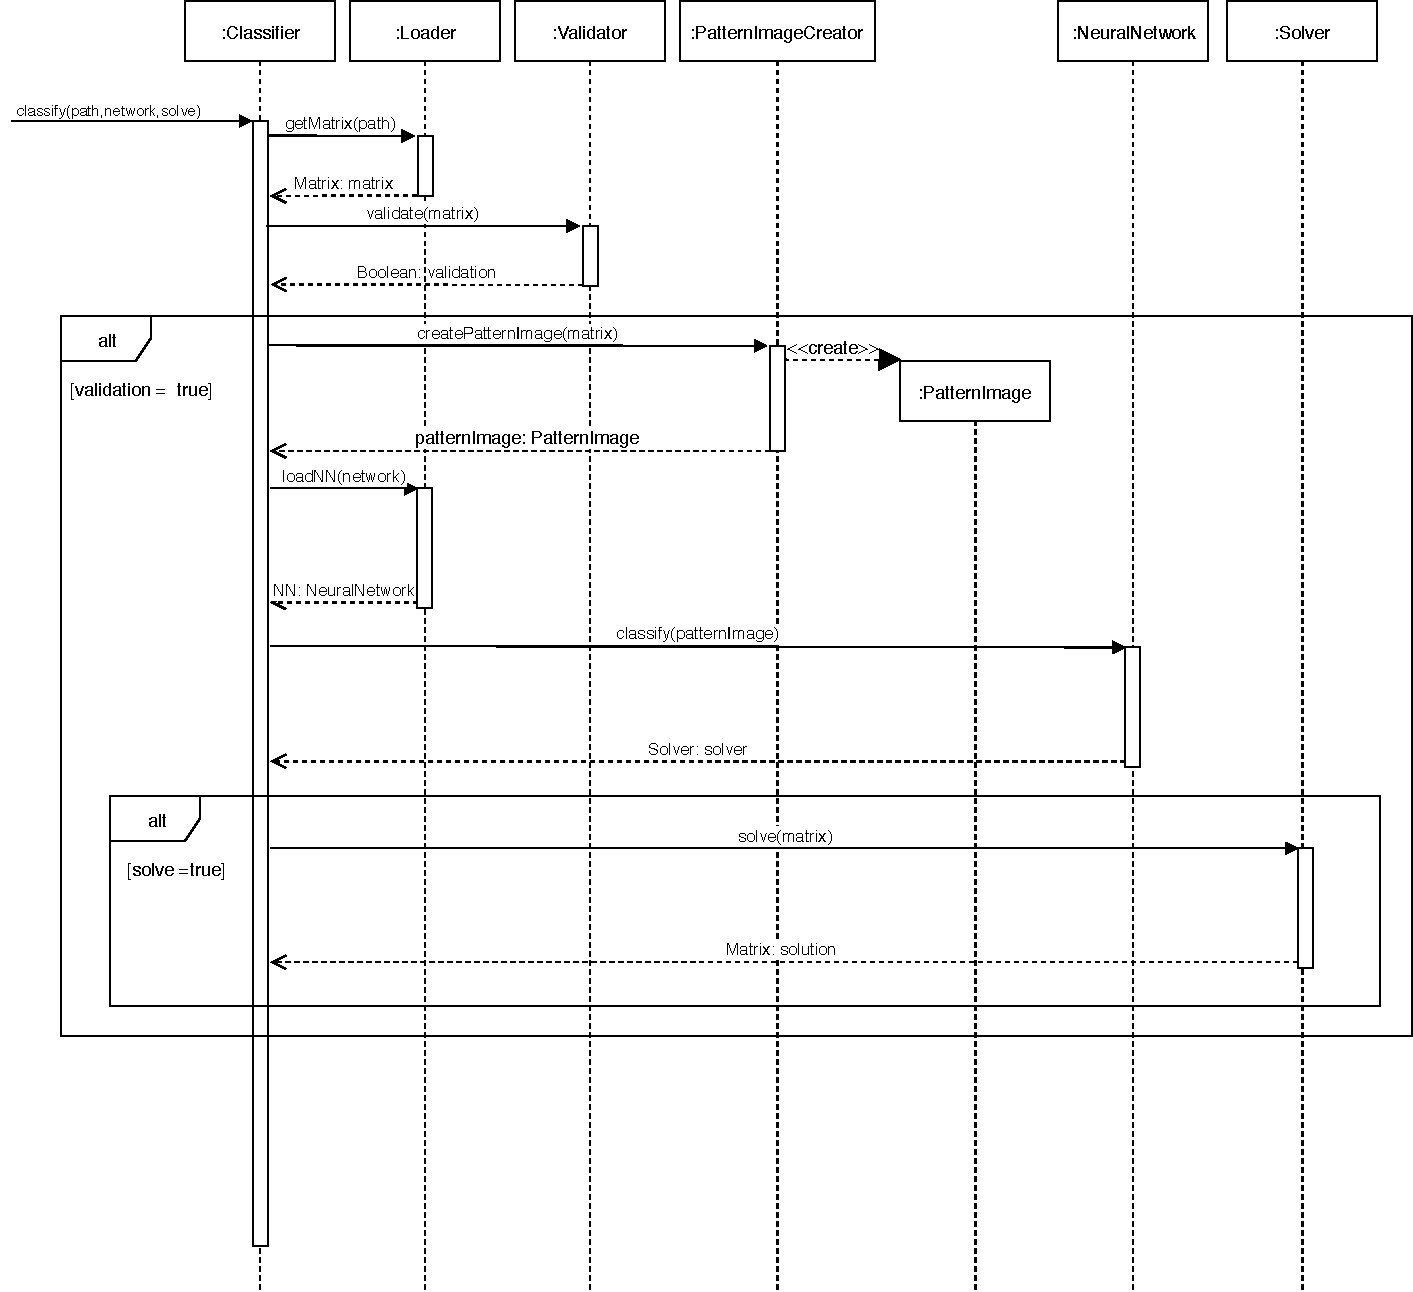
\includepdf[width=\textwidth]{SequenceDiagram/PDF/classifier_sequence_diagram}
\label{Sequence Diagrams}
\end{center}
\end{figure}

\newpage
\subsubsection{Description}
The method start has the input parameters "path" and "network".
The first parameter "path" is the path to the HDF5 file in which the matrix is saved that shall be classified.
The second parameter "network" is the path to the neural network which will classify the matrix.
First of all the classifier will be calling the Loader to load the Matrix.
The Loader will give back the matrix, that will be in the next step validated by the validator. 
The validator will give back a boolean value whether the matrix is regular (true) or not regular (false).
If the validation value is true the classifier will normalize the matrix. 
After that the matrix is normalized and ready for classification by the neural network.
So in the next step, the loader will load the neural network located on the given network path and gives back the neural network to the classifier.
In the next step, the classifier can give the matrix to the neural network for classification and the neural network gives back the  solver with which the matrix is classified.


\newpage
\section{Classes used by multiple modules}

\subsection{Class Loader}
\subsection{Class Saver}
The Saver class is just responsible for saving a given matrix dataset.
Its only method is the public method save(dataset: Dataset, name: String, path: String).
The save method takes a matrix dataset, converts it into an HDF5 file and saves it into a given directory with a given name.
\subsubsection{Activity Diagram}
\newpage
\begin{figure}[h]
\begin{center}
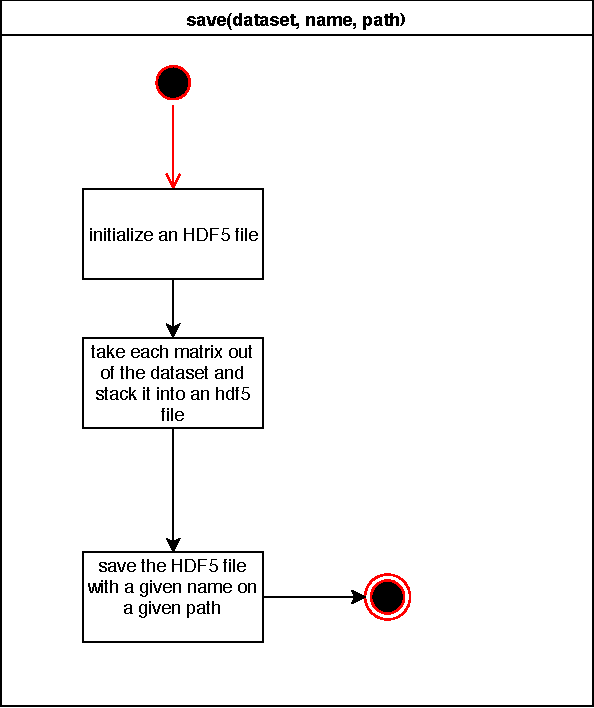
\includepdf[width=\textwidth, height= \textheight, keepaspectratio]{ActivityDiagrams/PDF/Collector_save_activity.pdf}
\label{Activity Diagrams}
\end{center}
\end{figure}
\newpage
This activity diagram shows how a dataset is saved with a given name on a given path. First of all an HDF5 file is initialized. After that each matrix is taken out of the dataset and stacked into the initialized HDF5 file, then the HDF5 file is saved with the given name on the given path.
\subsection{Class Validator}
The Validator class is a util class and responsible for validating given matrices(checking for regularity)
Its only static method validate takes a matrix and returns true for regular, and false for not regular.
\subsubsection{Activity Diagram}
\newpage
\begin{figure}[h]
\begin{center}
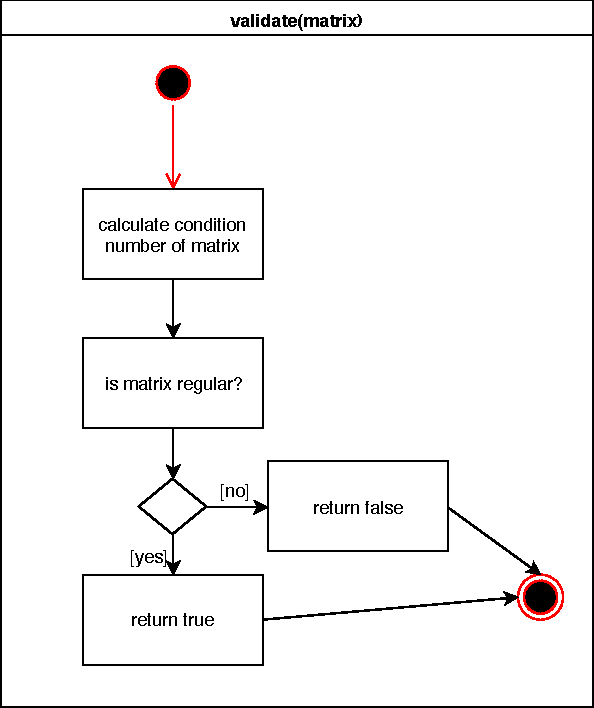
\includepdf[width=\textwidth, height= \textheight, keepaspectratio]{ActivityDiagrams/PDF/Collector_validate_activity.pdf}
\label{Activity Diagrams}
\end{center}
\end{figure}
\newpage

This activity diagram shows how a given matrix is validated. First the condition number of the matrix is calculated, when the condition number implies regularity, true is returned. Otherwise false is returned.

\subsection{Class Matrix}
The Matrix class is for representing matrices. It is defined by two attributes. The first attribute is the matrix size which is an integer and the second attribute are the matrix values which is a two-dimensional integer array. Both attributes are set with a constructor and can be requested by its get methods.

\subsection{Class Neural Network}


\newpage
\section{Glossary}
%\glspl{collector}, labeling modle, neural network, classifier, default settings  \glspl{Dateiformat}

% % Automatisch generiertes Glossar (Latex zwei mal ausführen um Glossar anzuzeigen)
%
%\glsaddall % das sorgt dafür, dass alles Glossareinträge gedruckt werden, nicht nur die verwendeten. Das sollte nicht nötig sein!
\printnoidxglossaries

\end{document}

